\documentclass[]{fairmeta}

% Shared style tweaks for clean references, tables, math, and lists
% Loaded by paper.tex after \documentclass

% Hyperlinks and smart cross-references
\usepackage{hyperref}
\usepackage{cleveref}

% Math & symbols
\usepackage{mathtools}
% High-quality math utilities: operators, paired delimiters, and shorthands
% Sets
\newcommand{\R}{\mathbb{R}}
\newcommand{\N}{\mathbb{N}}
\newcommand{\Z}{\mathbb{Z}}
% Operators
\DeclareMathOperator*{\argmin}{arg\,min}
\DeclareMathOperator*{\argmax}{arg\,max}
\DeclareMathOperator{\softmax}{softmax}
\DeclareMathOperator{\sgn}{sgn}
\DeclareMathOperator{\diag}{diag}
% Expectations / probabilities / information measures
\newcommand{\E}[2][]{\mathbb{E}_{#1}\!\left[\,#2\,\right]}
\newcommand{\Prob}[2][]{\mathbb{P}_{#1}\!\left( #2 \right)}
\newcommand{\Var}[2][]{\operatorname{Var}_{#1}\!\left[\,#2\,\right]}
\newcommand{\Cov}[2][]{\operatorname{Cov}_{#1}\!\left[\,#2\,\right]}
\newcommand{\KL}[2]{\operatorname{KL}\!\left(#1 \,\|\, #2\right)}
\newcommand{\TV}[2]{\operatorname{TV}\!\left(#1 , #2\right)}
% Paired delimiters (guarded to avoid redefinition if class provides them)
\makeatletter
\@ifundefined{abs}{\DeclarePairedDelimiter{\abs}{\lvert}{\rvert}}{}
\@ifundefined{norm}{\DeclarePairedDelimiter{\norm}{\lVert}{\rVert}}{}
\@ifundefined{ceil}{\DeclarePairedDelimiter{\ceil}{\lceil}{\rceil}}{}
\@ifundefined{floor}{\DeclarePairedDelimiter{\floor}{\lfloor}{\rfloor}}{}
\@ifundefined{set}{\DeclarePairedDelimiter{\set}{\lbrace}{\rbrace}}{}
\@ifundefined{paren}{\DeclarePairedDelimiter{\paren}{(}{)}}{}
\@ifundefined{bracket}{\DeclarePairedDelimiter{\bracket}{[}{]}}{}
\@ifundefined{inner}{\DeclarePairedDelimiterX{\inner}[2]{\langle}{\rangle}{#1,\,#2}}{}
\makeatother
% Differentials and linear algebra
\newcommand{\dd}{\mathop{}\!\mathrm{d}}
\newcommand{\grad}{\nabla}
\newcommand{\trans}{^{\mathsf{T}}}
% Definition/equality markers
\newcommand{\defeq}{\coloneqq}
\newcommand{\eqdef}{\eqqcolon}
% Lightweight bold vectors/matrices
\newcommand{\vct}[1]{\bm{#1}}
\newcommand{\mtx}[1]{\bm{#1}}
% Handy sequence shorthands
\newcommand{\xseq}{x_{1:T}}\newcommand{\aseq}{a_{1:T}}\newcommand{\zseq}{z_{1:T}}

% Numbers/units (alignment, ranges)
\usepackage{siunitx}
\sisetup{
  detect-all,
  group-separator = {,},
  group-minimum-digits = 4,
  per-mode = symbol,
  separate-uncertainty,
  table-number-alignment = center,
  table-text-alignment = center,
}

% Better tables
\usepackage[table]{xcolor}
\usepackage{tabularx}
\usepackage{array}
\usepackage{wrapfig}
\usepackage{ragged2e} % for \justifying in table cells
\usepackage{pdflscape}
\usepackage{float}
% L/C/R/Y provided by class; avoid redefining here
% Fully-justified fixed-width and auto-width columns
\newcolumntype{J}[1]{>{\justifying\arraybackslash}p{#1}}
\newcolumntype{Z}{>{\justifying\arraybackslash}X}
% Vertically center tabularx X-columns (and thus Z-columns)
\renewcommand\tabularxcolumn[1]{m{#1}}

% Metric and model names (small caps, consistent inline usage)
\newcommand{\PSNR}{\textsc{PSNR}}
\newcommand{\SSIM}{\textsc{SSIM}}
\newcommand{\LPIPS}{\textsc{LPIPS}}
\newcommand{\FVD}{\textsc{FVD}}

% Neural computer instances
\newcommand{\nccligen}{NC$_\text{CLIGen}$}
\newcommand{\ncguiworld}{NC$_\text{GUIWorld}$}

% Difficulty icon for CNC capability tables (medal graphic)
% Medal size (scaled up by 1.5x from the initial setting).
\newcommand{\cncmedal}{%
  \raisebox{0.25ex}{
\includegraphics[height=3.0ex]{assets/medal-removebg-preview.png}}%
}
\newcommand{\cncmedaltwo}{\cncmedal\cncmedal}
\newcommand{\cncmedalthree}{\cncmedal\cncmedal\cncmedal}
\newcommand{\cncmedalfour}{%
  \shortstack{\cncmedalthree\\[-0.7ex]\cncmedal}%
}
\newcommand{\cncmedalfive}{%
  \shortstack{\cncmedalthree\\[-0.7ex]\cncmedaltwo}%
}

% Tiny TikZ helper for experiment markers
\usepackage{tikz}
\usetikzlibrary{shapes}

% SVG figures (requires --shell-escape; used for some appendix diagrams)
\usepackage{svg}
\svgpath{{assets/}}

% Experiment headings: interface logo + bold title (logo optional)
\newcommand{\exptitle}[3][]{%
  \vspace{0.6em}%
  \noindent
  \ifstrempty{#1}{}{#1\hspace{0.5em}}%
  \textbf{Experiment~#2: #3}\par\vspace{0.25em}%
}

% Small helper for table footnotes
\newcommand{\tabnote}[1]{\vspace{2pt}{\raggedright\footnotesize #1\par}}

% Prompt-tier caption helper: label + horizontal rule
\newcommand{\prompttierline}[1]{%
  \noindent\textbf{#1}\hspace{0.5em}%
  \rule[0.55ex]{0.9\linewidth}{0.4pt}\par%
}

% Compact lists
\usepackage{enumitem}
\setlist[itemize]{noitemsep, topsep=2pt, leftmargin=1.2em}
\setlist[enumerate]{noitemsep, topsep=2pt, leftmargin=1.4em}

% Short, consistent cross-references via cleveref
\crefname{equation}{Eq.}{Eqs.}
\Crefname{equation}{Equation}{Equations}
\crefname{figure}{Fig.}{Figs.}
\Crefname{figure}{Figure}{Figures}
\crefname{table}{Tab.}{Tabs.}
\Crefname{table}{Table}{Tables}
\crefname{section}{Section}{Sections}


% Small helper for consistent small tables (only define if absent)
\makeatletter
\@ifundefined{smallschemetable}{%
  \newenvironment{smallschemetable}[2]{% caption, label
    \begin{table}[t]
      \centering
      \small
      \caption{#1}
      \label{#2}
  }{\end{table}}%
}{}%
\makeatother

% Definition boxes (for crisp model/spec statements)
% Requires tcolorbox (loaded by the class). Uses class colors.
% A lighter, cleaner style with subtle title pill and balanced spacing.
\newtcolorbox{defbox}[2][]{
  breakable,
  enhanced,
  colback=white,
  colframe=metablue!55,
  boxrule=0.6pt,
  arc=5pt,
  left=8pt, right=8pt, top=6pt, bottom=6pt,
  boxsep=2pt,
  before skip=8pt, after skip=8pt,
  title={#2},
  fonttitle=\sffamily\bfseries\small,
  coltitle=metafg,
  before upper={\parindent=0pt\justifying},
  attach boxed title to top left={yshift=-3pt,xshift=8pt},
  boxed title style={
    frame empty,
    colback=metablue!10,
    boxsep=2pt,
    left=6pt,right=6pt,top=2pt,bottom=2pt,
    arc=5pt
  }
}

% Compact compute/latency callout
\newenvironment{computebox}[1]{% title
  \begin{tcolorbox}[colback=metabg, colframe=metablue!40, arc=6pt, boxrule=0.4pt, left=6pt, right=6pt, top=6pt, bottom=6pt]
  {\sffamily\bfseries #1}\par\vspace{2pt}\small
}{\end{tcolorbox}}

% Optional placeholder figure macro (uniform look)
\newcommand{\phfig}[2][1.6in]{% height, note text
  \begin{tcolorbox}[colback=white, colframe=metablue!30, arc=6pt, boxrule=0.4pt]
    \centering
    \rule{0pt}{#1}\par\vspace{2pt}
    {\small #2}
  \end{tcolorbox}
}


\usepackage{caption}

\usepackage{xcolor}
\definecolor{mcwarm}{RGB}{150, 90, 60}
\newcommand{\mc}[1]{%
  {\color{mcwarm}\textsf{\small [Mingchen: #1]}}
}

\captionsetup{
  justification=raggedright,
  singlelinecheck=true
}
\usepackage{amssymb}

\providecommand{\blackstar}{\ensuremath{\bigstar}}
\providecommand{\blacklozenge}{\ensuremath{\lozenge}}
\providecommand{\spadesuit}{\textbf{+}}


\newcommand{\wenyi}[1]{\textcolor{red}{Wenyi: #1}}
\newcommand{\cligenGeneralLogo}{\raisebox{-0.18em}{
\includegraphics[height=1.0em]{assets/CLIGen_general.png}}}
\newcommand{\cligenCleanLogo}{\raisebox{-0.18em}{
\includegraphics[height=1.0em]{assets/CLIGEN_clean.png}}}
\newcommand{\guiworldLogo}{\raisebox{-0.12em}{
\includegraphics[height=1.0em]{assets/GUIWorld.png}}}
\newcommand{\cligenGeneralData}{\cligenGeneralLogo{}\,CLIGen (General)}
\newcommand{\cligenCleanData}{\cligenCleanLogo{}\,CLIGen (Clean)}
\newcommand{\guiworldName}{\guiworldLogo{}\,\ncguiworld{}}

% Custom (numeric) author markers
\DeclareRobustCommand{\MetaAffMark}{1}
\DeclareRobustCommand{\KaustAffMark}{2}
\DeclareRobustCommand{\CoreContribMark}{\textbf{+}}

\title{Neural Computers}

\author[\MetaAffMark,\KaustAffMark\CoreContribMark]{Mingchen Zhuge}
\author[\MetaAffMark\CoreContribMark]{Changsheng Zhao}
\author[\MetaAffMark,\KaustAffMark\CoreContribMark]{Haozhe Liu}
\author[\MetaAffMark\CoreContribMark]{Zijian Zhou}
\author[\MetaAffMark,\KaustAffMark\CoreContribMark]{Shuming Liu}
\author[\KaustAffMark]{Wenyi Wang}
\author[\MetaAffMark]{Ernie Chang}
\author[\MetaAffMark]{Gael Le Lan}
\author[\MetaAffMark,\KaustAffMark]{Junjie Fei}
\author[\MetaAffMark,\KaustAffMark]{Wenxuan Zhang}
% \author[\KaustAffMark]{Yasheng Sun}
\author[\MetaAffMark]{Yunyang Xiong}
\author[\MetaAffMark]{Zechun Liu}
\author[\MetaAffMark]{Zhipeng Cai}
\author[\MetaAffMark]{Yining Yang}
\author[\MetaAffMark]{Yuandong Tian}
\author[\MetaAffMark]{Yangyang Shi}
\author[\MetaAffMark]{Vikas Chandra}
\author[\KaustAffMark]{Jürgen Schmidhuber}
\affiliation[\MetaAffMark]{Meta AI}
\affiliation[\KaustAffMark]{KAUST}
\contribution[\textbf{+}]{Core Contributors}

\abstract{% We propose a new frontier: neural computers (NCs)—learned, executable runtimes—toward “living computers” that learn interface dynamics from experience.  
% We call the long-term goal a Completely Neural Computer (CNC): a single learned model of a computer that subsumes the classical compute/memory/I/O stack, thereby challenging the layered OS/application architecture that mediates I/O.
% As an initial step toward this vision, we ask whether a neural model can learn computer interface dynamics from collected I/O samples.
% We instantiate NCs as video models that roll out screen frames from instructions, recent pixels, and (when available) user actions, without access to instrumented program state.
% We conduct experiments in both CLI and GUI settings and derive practical design considerations for building CNCs.
% Finally, rather than imitating human or animal cognition, we ask whether neural networks can be designed to mirror the computational structure of machines—like circuit-based computers—and thereby go beyond both current foundation models and conventional computers.



We propose a new frontier: Neural Computers (NCs)—neural networks that unify computation, memory, and I/O in a single latent runtime state.
Our long-term goal is the Completely~Neural~Computer (CNC), the fully realized form of this vision: a general-purpose neural computer that challenges the layered architecture of conventional computers.
As an initial step, we study whether such executable dynamics can be learned~solely~from collected I/O traces, without access to instrumented program state.
Concretely, we instantiate NCs as video models that roll out screen frames conditioned on instructions, pixels, and (when available) user actions, and evaluate them in both CLI~and~GUI~settings.
We outline a roadmap toward CNCs, centered on fundamental challenges. 
If achieved, CNCs could inaugurate a new computing paradigm beyond both today’s foundation models and conventional~computers.
}

\date{\today}
\correspondence{\email{mczhuge@gmail.com, cszhao@meta.com}}

% You can add additional metadata fields as follows 
% \metadata[Code]{\url{https://github.com/metauto-ai/neuralcomputer}}
\metadata[Blogpost]{\url{https://metauto.ai/neuralcomputer}}

% Style helpers moved to assets/paperstyle for consistency

\begin{document}

\maketitle

\vspace{1.2em}
{\captionsetup{skip=2pt,font=footnotesize}}
\begin{figure}[H]
  \centering
  \hypertarget{teaser}{}
  
\includegraphics[width=0.92\linewidth]{assets/teaser10.pdf}
\end{figure}\label{fig:nc_teaser}
\vspace{-1.2em}
\begingroup
\setcounter{tocdepth}{1}
\vspace{-0.6em}
\small\normalfont
\renewcommand{\baselinestretch}{0.8}\selectfont
\setlength{\parskip}{0pt}
\setlength{\parindent}{0pt}
\vspace{-0.6em}
\tableofcontents
\endgroup

\newpage
\section{Introduction}
\label{section:intro}
Can a single set of weights act as a ``computer''?  
We term this abstraction a Neural Computer (NC): a neural network that models computer interface dynamics learned from experience.
% An NC couples environment dynamics, working memory, and interface I/O through pixels, actions, and language.
% In this paper, we train neural networks (NNs) to learn the dynamics of traditional computers (TCs). The NN's inputs include screenshots, instructions (natural language or program commands), and user actions such as keyboard typing and mouse movements/clicks.


To implement this idea, we instantiate NCs as video models.
Several lines of evidence suggest that, at this stage, video models are the most practical substrate for prototyping this vision—though we expect the long-term solution to require a fundamentally new neural architecture (\Cref{section:toward-cnc}).
%
This choice builds on perspectives like world models~\citep{ha2018world}, which demonstrate that neural networks can internalize environment dynamics and support predictive imagination; 
and advances in high-capacity video generators such as Veo~3.1~\citep{google_veo3_1_2025} and Sora~2~\citep{openai_sora2_2025} show that such learned dynamics can be rendered into coherent, photorealistic frame sequences; besides, 
frontier interactive video models such as Genie~3~\citep{bruce2024genie} further extend this trajectory, demonstrating action-controllable generative environments.
% 
In parallel, LLM-driven UI systems such as Imagine with Claude\footnote{\url{https://claude.ai/imagine/}} map natural-language inputs to structured interface updates. 
%` 
Yet these capabilities remain split across components: models~render~or~predict, while an external execution environment (simulator/OS/DOM) carries executable state and mediates control.

%To address this gap, we define a neural computer (NC) as a learned, executable, and ultimately programmable system in which the model, environment, and runtime share a unified latent state. An NC exposes a computer-like interface through pixels, actions, and language. 
We study two interfaces that instantiate our NC formulation (see ~\Cref{section:prelim}). 
\nccligen{} is a terminal interface conditioned on text (natural language or command lines) and an initial frame (\Cref{section:impl-cligen}). 
\ncguiworld{} is a desktop interface conditioned on recent pixels and synchronized mouse/keyboard actions (\Cref{section:impl-guiworld}).  
% 

\begin{tcolorbox}[
  colback=metablue!8,
  colframe=metablue!40,
  boxrule=0pt,
  borderline west={1pt}{0pt}{gray!60},
  left=6pt,right=4pt,top=3pt,bottom=3pt]
\small
\textbf{Neural Computer (NC) abstraction~(\hyperlink{teaser}{Teaser}).}
A neural system $(F, G)$ parameterized by $\theta$ that models the dynamics of an interactive computer interface 
% (iii) renders and controls the interface via pixels and actions
with a single latent runtime state $h_t$ that acts as its working memory (see~\cref{eq:wm}).
\end{tcolorbox}


In the \nccligen{} experiments, the NC can render and execute basic command-line workflows.
It often stays aligned with the terminal buffer and captures common ``physics'' of everyday CLI use (e.g., fast scrollback, prompt wrapping, window resizing).
On carefully scripted data, rollouts can be visually and structurally close to real sessions.
The model can execute short command chains and render their outputs.
Arithmetic-probe scores improve substantially with stronger system-level conditioning.
%Reprompting boosts probe accuracy from 4\% to 83\% (\Cref{fig:cligen-exp6}).

In the \ncguiworld{} experiments, we evaluate standard world-model designs across action injection, action encoding, and data quality.
Figure~\ref{fig:nc-general} summarizes this design template across two interface-specific NCs trained separately without shared parameters.
Qualitatively, the model learns coherent pointer dynamics and short-horizon action responses (e.g., hover/click feedback and window/menu transitions).
%With explicit cursor supervision, it reaches 98.7\% cursor accuracy (\Cref{tab:cursor-loss}).

Our experimental insights indicate that current NCs already realize several primitives of conventional computers, most notably I/O alignment and short-horizon control.
We define the long-term goal, a Completely Neural Computer (CNC), as a fully learned computer whose compute, memory, and interfaces are unified in a single learned runtime substrate rather than engineered as separate modules.
However, these prototypes represent only an early step toward this CNC vision.
Substantial challenges remain in achieving robust long-horizon reasoning, reliable symbolic processing, and stable interface rendering.
\Cref{section:toward-cnc} presents a CNC capability map and outlines key open challenges toward the CNC vision. 

\begin{tcolorbox}[
  colback=metablue!8,
  colframe=metablue!40,
  boxrule=0pt,
  borderline west={1pt}{0pt}{gray!60},
  left=6pt,right=4pt,top=3pt,bottom=3pt]
\small
\textbf{Completely Neural Computer (CNC) abstraction~(\Cref{sec:roadmap}).}
A Neural Computer instance is \emph{complete} (i.e., a CNC) if it is
(i) \emph{Turing complete},
(ii) \emph{universally programmable},
(iii) \emph{behavior-consistent} unless explicitly reprogrammed, and
(iv) realizes the architectural and programming-language semantics of NCs relative to conventional computers.
\end{tcolorbox}

\textbf{Concretely, this work makes the following contributions:}
{
\renewcommand\labelitemi{\large$\bullet$}
\begin{itemize}
\setlength{\itemsep}{2pt plus 1pt minus 1pt}
\setlength{\parskip}{0pt}
\item Define neural computers (NCs) and build video-based prototypes for both CLI and GUI interfaces.
% \item Release open-source video datasets spanning thousands of hours across both domains.
\item Provide a data engine and alignment recipe that synchronize text, actions, and frames~for~CLI and~GUI~environments.
\item Identify practical design choices for NCs through extensive ablation studies.
\item Outline a roadmap toward completely neural computers (CNCs) grounded in primitives of conventional computers and open research questions.

\end{itemize}
}


\section{Preliminaries}
\label{section:prelim}

Throughout this paper, we use \emph{conventional digital computers} as an umbrella term for stored-program machines (e.g., von Neumann-style architectures): at the theory level they are commonly abstracted as random-access machines with an instruction set architecture, and at the systems level they are typically realized through layered operating-system/application stacks. Such systems separate computation, memory, and I/O.
Our motivating question is whether a single set of weights can internalize these roles inside one latent runtime state, rather than relying on an external execution environment (e.g., OS/simulator) to carry executable state.
We model a video-based neural computer (NC) prototype as a learned latent-state system that folds these roles into an update-and-render loop.

\begin{figure}[h!]
  \centering
  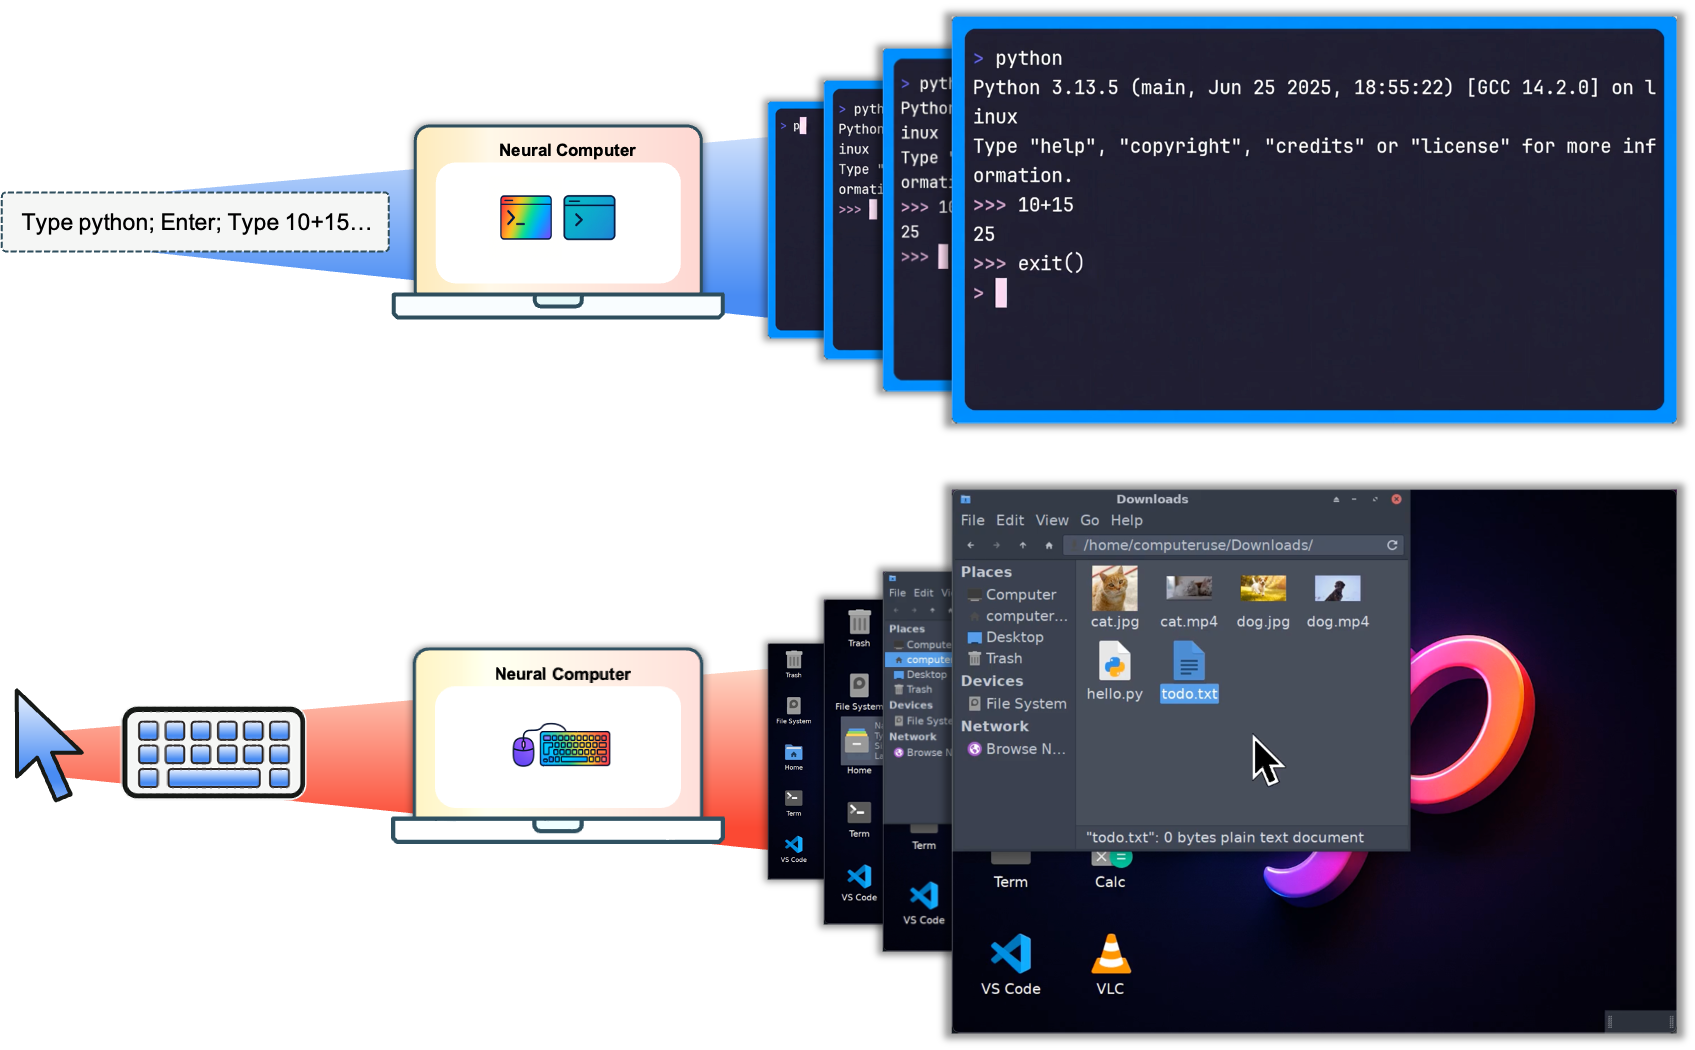
\includegraphics[width=1.0\linewidth]{assets/nc_general.png}
\caption{\textbf{Neural computers across interfaces.}
Given a prompt or action stream, an NC rolls out future interface frames for \cligenGeneralLogo{}/\cligenCleanLogo{}\,\nccligen{} (top) and \guiworldLogo{}\,\ncguiworld{} (bottom).
Logos denote datasets; \nccligen{} and \ncguiworld{} are the corresponding models trained on those datasets.
It models terminal or desktop dynamics.}
  \label{fig:nc-general}
\end{figure}

Specifically, an NC updates a latent runtime state from the current observation and conditioning input, and then predicts (or samples) the next observation.
In this paper, we treat screen frames as observables and define actions as time-indexed conditions. More broadly, the NC framework can accommodate various other modalities and structural representations for both observables and actions.
Given an initial screen frame $x_0$ and conditioned on user action $u_t$ at iteration $t$, an NC updates its memory state and samples the next frame $x_{t+1}$.
% Formally, an NC defined by an initial memory state $h_0$, an update function $F_\theta$, and a decoder $G_\theta$ operates as follows:
Formally, an NC defined by an initial memory state $h_0$, an update function $F_\theta$, and a decoder $G_\theta$ operates as follows, where $G_\theta$ parameterizes a distribution over next frames:


\begin{align}
h_t &= F_\theta(h_{t-1}, x_t, u_t), \qquad x_{t+1} \sim G_\theta(h_t).
\label{eq:wm}
\end{align}

\noindent\textit{Notation.} We use $h_t$ for the NC latent runtime state and reserve $z$ for VAE/video latents used in diffusion-style video models (e.g., \Cref{section:impl-guiworld}). 

We cast this update-and-render loop as a world model of a computer interface, where $x_t$ are observations and $u_t$ provides conditioning.
In world-modeling terminology, the input sequence $\{u_t\}$ is referred to as a conditioning stream.
Under this view, an NC is not merely a predictor but a learned runtime mechanism: the latent state $h_t$ carries executable context; $F_\theta$ integrates new observations and inputs, and $G_\theta$ renders the next frame.
Auxiliary heads can encode and decode prompts, buffers, or action traces, shifting functionality that would traditionally live in OS queues, device drivers, and UI toolkits into latent-state dynamics.

\subsection{Related Work}
\label{section:prelim-related}

Early neuromorphic designs~\citep{mead2012analog} explored neural computation as a physical substrate.
Differentiable memory and program-execution architectures, including Neural Turing Machines~\citep{graves2014neural},
Differentiable Neural Computers~\citep{graves2016hybrid}, and Neural Programmer-Interpreters~\citep{reed2015neural}, showed that neural controllers with memory can execute structured procedures.
Differentiable world models~\citep{schmidhuber1990making,schmidhuber2015learning} learn neural representations of environment dynamics, and inspire our update-and-render formulation.
%
Latent video and world models~\citep{ha2018world,hafner2019learning,hafner2019dream,bruce2024genie} extend these ideas to embodied control and interactive environments.
Genie~3~\citep{bruce2024genie}, in particular, frames such models as agent-training substrates with improved physical consistency.
More recently, high-capacity generators such as Veo~3~\citep{google_veo3_1_2025} and Sora~2~\citep{openai_sora2_2025} emphasize open-ended, photorealistic simulation.
In parallel, systems such as NeuralOS~\citep{rivard2025neuralos} and Imagine with Claude~\citep{anthropic_claude_sonnet4_5_2025} bring model-based conditioning to desktop and DOM-style interfaces.
%
Building on this trajectory, we study two NC instantiations for CLI and GUI with interface-specific conditioning, supported by a shared data engine and a staged roadmap toward the CNC vision.


\section{Implementation of Neural Computers}
\label{section:implementation}

\begin{figure}[t]
  \centering
  \makebox[\linewidth][c]{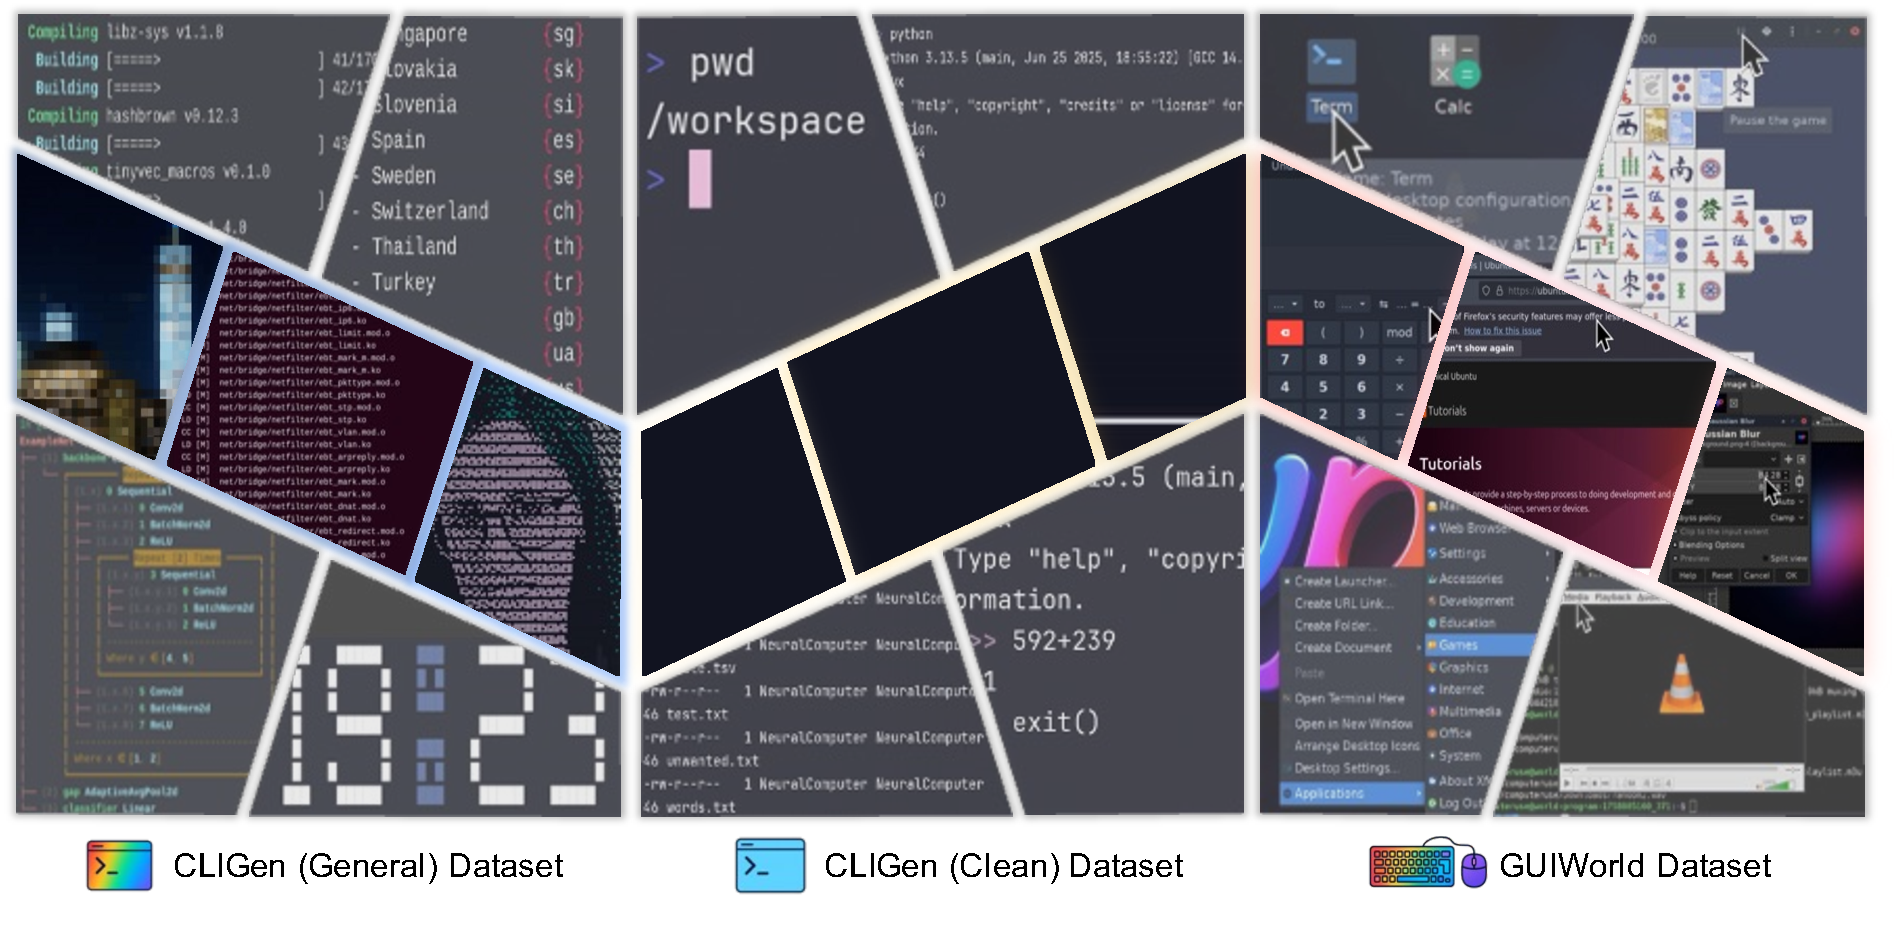
\includegraphics[width=1.15\linewidth]{assets/data_teaser9.pdf}}
  \caption{\textbf{Data types used to learn NC behaviors.} Logos denote datasets: \cligenGeneralLogo{}\,CLIGen (General) replays public \texttt{asciinema} traces spanning diverse real-world terminal workflows. \cligenCleanLogo{}\,CLIGen (Clean) uses scripted \texttt{vhs} runs to capture deterministic terminal traces for controlled experiments. \guiworldLogo{}\,GUIWorld captures desktop RGB with synchronized mouse/keyboard traces to validate action-conditioned rendering and control on GUIs.}
  \label{fig:data-teaser}
\end{figure}



We build on the Wan2.1 model~\citep{wan2025wan}, which was a state-of-the-art video generation model at the time of our experiments.
We add NC-specific conditioning and action modules, together with interface-specific training recipes.
Figure~\ref{fig:nc-general} illustrates this setup: NCs take a prompt or action stream as input and generate future interface frames in both CLI and GUI settings.
We refer to these two instantiations as CLIGen (CLI; \Cref{section:impl-cligen}) and GUIWorld (GUI; \Cref{section:impl-guiworld}).

In this video-based instantiation, we implement the NC latent runtime state $h_t$ using the model’s time-indexed latent representations $z_t$.
This abstracts the underlying diffusion transformer as a latent dynamical system.
The transformer $F_\theta$ maps prior context and current observations/conditioning into an updated state $h_t$ (realized as $z_t$).
The decoder $G_\theta$ parameterizes a distribution over the next frame $x_{t+1}$.
Auxiliary heads encode and decode conditioning streams $u_t$, including text prompts and action traces.
Structured logs such as terminal buffers are used for alignment and evaluation where available, not as privileged model-state inputs.


\subsection{\cligenGeneralLogo{}\,/\,\cligenCleanLogo{}\,\,The CLI Video Generators}
\label{section:impl-cligen}


CLIGen instantiates the NC abstraction in command-line interfaces.
Observations $x_t$ are terminal frames rendered from the underlying text buffer.
The conditioning stream $u_t$ carries a user prompt and optional metadata, and the video latent state $z_t$ implements the latent runtime state $h_t$ by tracking CLI context across frames.
At inference time, the model rolls out from the prompt and first frame, updates $z_t$, and predicts future terminal frames (\Cref{fig:cligen-arch}).
Throughout this section, \cligenGeneralLogo{}\,CLIGen (General) and \cligenCleanLogo{}\,CLIGen (Clean) denote datasets, and we train one \nccligen{} model per dataset under the same architecture.



\newcommand{\dsrow}[2]{%
  \noindent\makebox[0.72\linewidth][l]{#1}%
  \makebox[0.26\linewidth][r]{#2}\par
}

\begin{tcolorbox}[
  colback=metablue!8,
  colframe=metablue!40,
  boxrule=0pt,
  borderline west={1pt}{0pt}{gray!60},
  left=6pt,right=4pt,top=3pt,bottom=3pt]
\small
\textbf{Datasets $\leftrightarrow$ models.}
\begin{itemize}
  \setlength{\itemsep}{2pt}
  \setlength{\topsep}{2pt}
  \item \cligenGeneralLogo{}\,\text{CLIGen (General)}: diverse, open-ended terminal traces.\hfill
        \textit{Model:} \cligenGeneralLogo{}\,\nccligen{}
  \item \cligenCleanLogo{}\,\text{CLIGen (Clean)}: deterministic Dockerized scripts with cleaner, better-paced buffers.\hfill
        \textit{Model:} \cligenCleanLogo{}\,\nccligen{}
\end{itemize}
\end{tcolorbox}


 

\newcommand{\cliframe}[2]{%
  \begin{tikzpicture}[baseline={(current bounding box.center)}]
    \node (img) [inner sep=0pt] {\includegraphics[width=0.34\linewidth,keepaspectratio]{#1}};
    \node[anchor=south east, fill={rgb,1:red,0.98;green,0.91;blue,0.73}, text=black, circle, inner sep=2pt] at ([xshift=-4pt,yshift=4pt]img.south east) {\scriptsize #2};
  \end{tikzpicture}%
}
\newcommand{\cliframeblock}{%
  \makebox[\linewidth][c]{%
    \begingroup
    \setlength{\tabcolsep}{0.26em}% slightly larger horizontal gap
    \renewcommand{\arraystretch}{1.0}%
    \begin{tabular}{ccc}
      \cliframe{assets/sample1}{1} & \cliframe{assets/sample2}{2} & \cliframe{assets/sample3}{3} \\
      \addlinespace[0.48em]% slightly larger vertical gap
      \cliframe{assets/sample4}{4} & \cliframe{assets/sample5}{5} & \cliframe{assets/sample6}{6}
    \end{tabular}%
    \endgroup}}

% Clean sample frames (CLIGen Clean)
\newcommand{\cliframeclean}[2]{%
  \begin{tikzpicture}[baseline={(current bounding box.center)}]
    \node (img) [inner sep=0pt] {\includegraphics[width=0.34\linewidth,keepaspectratio]{#1}};
    \node[anchor=south east, fill={rgb,1:red,0.98;green,0.91;blue,0.73}, text=black, circle, inner sep=2pt] at ([xshift=-4pt,yshift=4pt]img.south east) {\scriptsize #2};
  \end{tikzpicture}%
}
\newcommand{\cliframecleanblock}{%
  \makebox[\linewidth][c]{%
    \begingroup
    \setlength{\tabcolsep}{0.26em}% match horizontal gap
    \renewcommand{\arraystretch}{1.0}%
    \begin{tabular}{ccc}
      \cliframeclean{assets/sample1_cligen}{1} & \cliframeclean{assets/sample2_cligen}{2} & \cliframeclean{assets/sample3_cligen}{3} \\
      \addlinespace[0.48em]% match vertical gap
      \cliframeclean{assets/sample4_cligen}{4} & \cliframeclean{assets/sample5_cligen}{5} & \cliframeclean{assets/sample6_cligen}{6}
    \end{tabular}%
    \endgroup}}

\begin{smallschemetable}{Data samples for \cligenGeneralLogo{}\,CLIGen (General) and \cligenCleanLogo{}\,CLIGen (Clean).}{tab:cligen-prompts}
  \begin{tabularx}{\linewidth}{X}
    \multicolumn{1}{c}{\textbf{Frames from Sample — \cligenGeneralLogo{}\,CLIGen (General)}}\\[0.25em]
    \multicolumn{1}{c}{\cliframeblock}\\[7.0em]
    \noalign{\vspace{0.9em}}
    \makebox[\textwidth][c]{\parbox{1.01\textwidth}{%
    \prompttierline{Semantic}
    A root terminal session kicks off an AI command to make three 1024x1024 cat shots, shows quick parsing for each one, then presents pixelated cat previews with numbered links and asks whether to stash them in \texttt{/root/2023\_04\_01-02\_27\_11\_imgs}. \par\medskip
	    \prompttierline{Regular}
	    In a root shell at \texttt{\texttildelow}, the user runs \texttt{ai -i 3 a cute cat}, watches a green progress line announcing three 1024x1024 images, sees sequential parsing messages for images 1 through 3, and ends on a preview pane with three pixelated cat thumbnails, numbered download links, and a save prompt targeting \texttt{/root/2023\_04\_01-02\_27\_11\_imgs}. \par\smallskip
	    \prompttierline{Detailed}
	    In a dark-background terminal at the \texttt{root in \texttildelow} prompt, the user types \texttt{ai -i 3 a cute cat}. The screen prints \texttt{Generating 3 1024x1024 images (press CTRL-C to cancel)...}, shows parsing messages for images 1--3, and ends on a preview pane with three numbered thumbnails and a save prompt targeting \texttt{/root/2023\_04\_01-02\_27\_11\_imgs}.}}\\[0.7em]
    \midrule
    \multicolumn{1}{c}{\textbf{Frames from Sample — \cligenCleanLogo{}\,CLIGen (Clean)}}\\[0.25em]
    \multicolumn{1}{c}{\cliframecleanblock}\\[6.2em]
    \noalign{\vspace{0.6em}}
    \makebox[\textwidth][c]{\parbox{1.01\textwidth}{%
    \prompttierline{Scripted caption}
    Type \texttt{python}; Enter; Type \texttt{values = [n*n for n in range(1, 10)]}; Enter; Type \texttt{print(values)}; Enter; Type \texttt{exit()}; Enter.}}\\
  \end{tabularx}
\end{smallschemetable}





\subsubsection{Data pipeline}

The \cligenGeneralLogo{}\,CLIGen (General) dataset is built from publicly available \texttt{asciinema .cast} trajectories\footnote{\url{https://asciinema.org/}}.
The \texttt{asciinema} stack records and replays terminal sessions with synchronized timing and ANSI-faithful decoding.
We replay each session with the official tools and render it into terminal frames, preserving palette transitions, cursor state, and terminal geometry.
Frames, text buffers, and keyboard-event logs share a single monotonic clock.
At render time, we normalize resolution and aspect ratio and apply a filter to remove sensitive strings.
We render sessions to GIF using \href{https://github.com/asciinema/agg}{\texttt{agg}} and convert them to video with \href{https://github.com/FFmpeg/FFmpeg}{\texttt{ffmpeg}}.

We segment each recording into roughly five-second clips using content-aware splits. 
We temporally normalize each clip to a fixed length: shorter clips repeat the final frame, and longer clips are uniformly subsampled. 
The resulting 823{,}989 video streams (approximately 1{,}100 hours) are resampled to 15~FPS.
Underlying buffers and logs are used to generate aligned textual descriptions with Llama~3.1~70B~\citep{dubey2024llama} in three styles (semantic, regular, and detailed), which serve as prompts.
As shown in Figure~\ref{fig:data-teaser} (left), this split spans diverse real-world terminal use cases\footnote{Additional preprocessing details and a \texttt{.cast} example are in \Cref{appendix:pipeline,appendix:cast-format}, with a sample overview in \Cref{tab:cligen-prompts}.}.







The \cligenCleanLogo{}\,CLIGen (Clean) dataset is collected using the open-source \href{https://github.com/charmbracelet/vhs}{\texttt{vhs}} toolkit.
It enables repeatable terminal demonstrations and integration tests through scripted execution.
Deterministic scripts drive Dockerized environments to capture cleaner, better-paced traces.
We authored roughly $250$k scripts.
After filtering (51.21\% retained), we keep two subsets.
The first contains approximately $78$k regular traces (package installation, log filtering, interactive REPL usage, etc.).
The second contains approximately $50$k Python math validation traces.
Captions are derived directly from the raw \texttt{vhs} scripts for clarity.
We standardize frame rendering by fixing one monospace font/size, using a consistent palette for success and error highlights, and locking resolution and theme to remove typography-related confounds.
Each episode records its caption type and font settings for later slicing.
Clips longer than five seconds are uniformly subsampled for training, while shorter clips repeat the final frame to normalize length\footnote{Additional details are provided in \Cref{appendix:pipeline,appendix:vhs-format}, with a representative data sample in \Cref{tab:cligen-prompts}.}.



\subsubsection{Model architecture}

We treat CLI generation as text-and-image-to-video: a caption and the first terminal frame condition the rollout.
The first frame is encoded by a VAE into a conditioning latent.
In parallel, a CLIP image encoder~\citep{radford2021learning} extracts visual features from the same frame, and a text encoder (e.g., T5~\citep{raffel2020exploring}) embeds the caption.
Following the Wan2.1 image-to-video (I2V) design, these conditioning features are concatenated with diffusion noise, projected through a zero-initialized linear layer, and processed by a DiT stack.
Decoupled cross-attention injects the joint caption and first-frame context derived from the CLIP and text features. 
%
The VAE encodes and decodes terminal frames.
During generation, the diffusion transformer advances the latent state $z_t$ under the original Wan2.1 I2V sampling schedule, without additional binary masks or periodic reseeding.



\begin{figure}[ht]
  \centering
  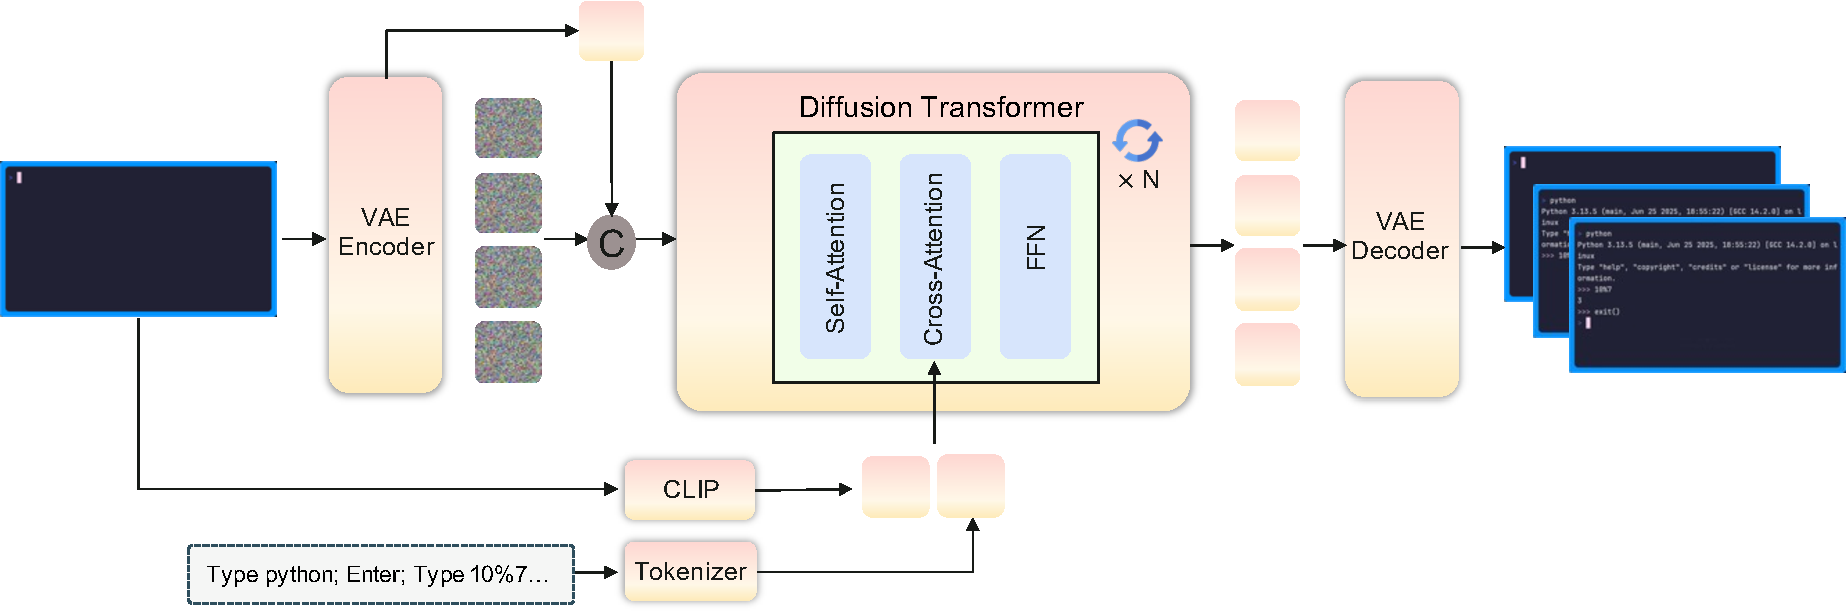
\includegraphics[width=0.8\linewidth]{assets/cligen_7}
  \caption{\cligenGeneralLogo{}\,/\,\cligenCleanLogo{}\,NC$_\text{CLIGen}$ architecture.
  Terminal frames are observations $x_t$.
  A prompt and the first frame seed the conditioning stream.
  The Wan2.1-based latent state $z_t$ rolls forward under the standard I2V sampling scheme.}
  \label{fig:cligen-arch}
\end{figure}






\subsubsection{Implementation Details}

Training uses gradient checkpointing and applies dropout 0.1 to the prompt encoder, CLIP, and VAE modules.
Optimization uses AdamW (learning rate $5\times10^{-5}$, weight decay $10^{-2}$), \texttt{bfloat16} precision, and gradient clipping at 1.0.
%
Training \nccligen{} on CLIGen (General) requires $\sim$15{,}000 H100 GPU hours at batch size 1.
Training on CLIGen (Clean) across both subsets requires $\sim$7{,}000 H100 GPU hours.


\subsubsection{Evaluations}

% Our CLI neural computer achieves high-fidelity rendering and basic interaction.
Unless otherwise noted, NC in this section refers to the current video-based CLI prototype. We report six practical takeaways:
\begin{tcolorbox}[
  colback=metablue!6,
  colframe=metablue!40,
  boxrule=0pt,
  borderline west={1pt}{0pt}{gray!60},
  left=6pt,right=4pt,top=3pt,bottom=3pt]
\small
\begin{itemize}
  \setlength{\itemsep}{3pt}
  \setlength{\topsep}{2pt}
  \item The NC maintains high-fidelity terminal rendering at practical font sizes (e.g., 13\,px), preserving readable interface state.
  \item Prompt specificity is an effective control channel: detailed, literal captions improve text-to-pixel alignment.
  \item On clean but domain-specific data, PSNR/\SSIM~plateau around 25k steps (Figure~\ref{fig:cligen-long-train}), suggesting coverage matters more than longer optimization.
  \item The NC reproduces complex terminal appearances while sustaining multi-step command execution.
  \item Symbolic computation remains the main bottleneck: structured arithmetic reveals reliability limits, motivating stronger symbolic or system-level conditioning.
  \item In our setting, without changing the NC backbone or adding RL, reprompting improves symbolic probes (4\%$\rightarrow$83\%; Figure~\ref{fig:cligen-exp6}), supporting the view that current models are strong renderers but not reasoners (Table~\ref{tab:sora-leads}).
\end{itemize}
\end{tcolorbox}


\exptitle[\cligenGeneralLogo]{1}{The NC stays readable at practical font sizes}


Concurrent work~\citep{rivard2025neuralos} argues that generic natural-image VAEs can perform poorly on structured computer screenshots.
We test this claim directly by applying the Wan2.1 VAE~\citep{wan2025wan} to terminal content.
In our setting, reconstruction quality is primarily governed by font size.
At 13\,px, it is high (40.77\,dB \PSNR, 0.989 \SSIM).
At 6\,px, text exhibits noticeable blurring even when global \PSNR/\SSIM~remain strong, because background regions dominate these metrics.


\begin{figure}[h!]
  \centering
  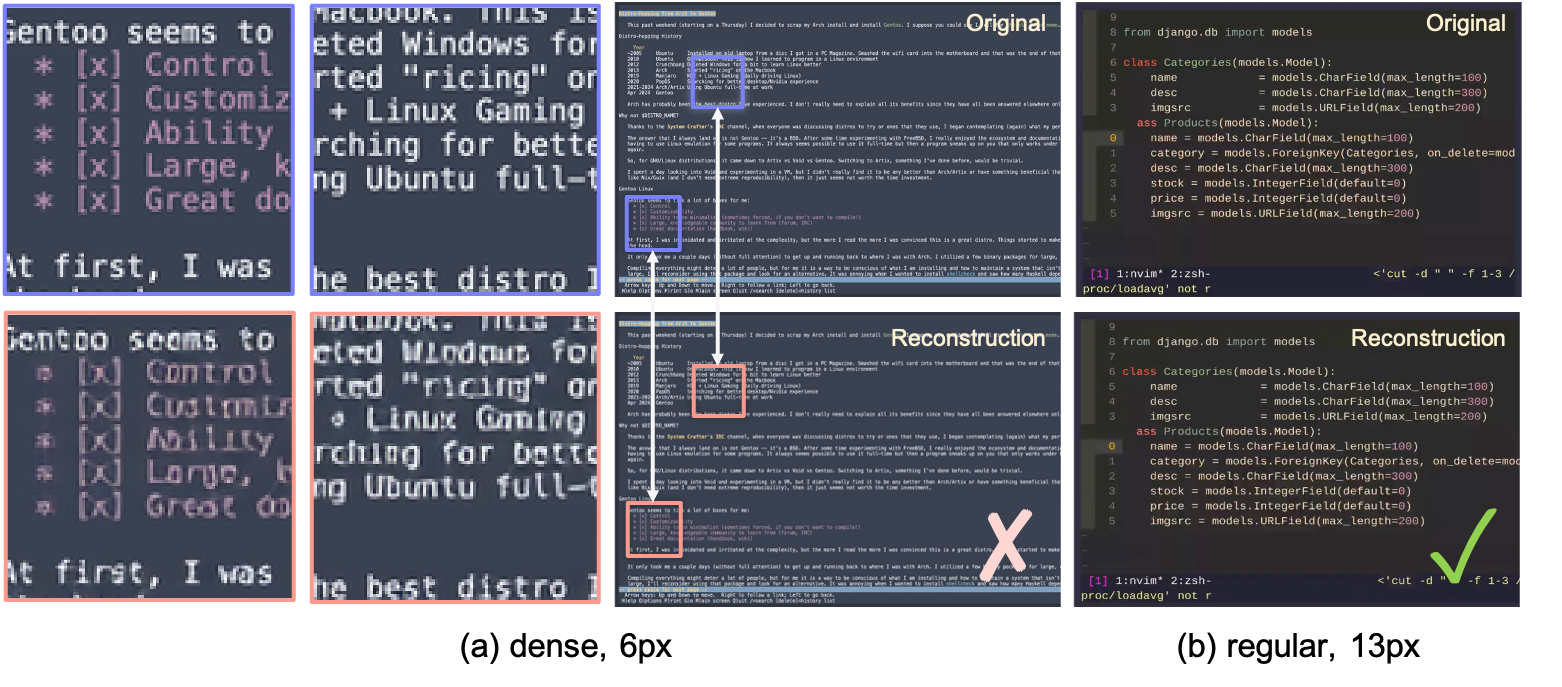
\includegraphics[width=\linewidth]{assets/recon_comp3.png}
    \vspace{-15pt}
\caption{Wan2.1 VAE reconstructions on CLIGen (General) terminal frames at different font sizes.}
  \label{fig:cligen-exp1}

\end{figure}


\begin{wraptable}{r}{0.42\linewidth}
  \vspace{-22pt}
  \captionsetup{type=table,width=\linewidth}
  \centering
  \small
  \rowcolors{2}{metablue!8}{white}
  \caption{Reconstruction quality.}
  \label{tab:cli-vae-recon}
  \setlength{\tabcolsep}{7pt}
  \begin{tabularx}{\linewidth}{l >{\centering\arraybackslash}X}
    \toprule
    \rowcolor{metablue!16} \textbf{Metric} & \textbf{Value} \\
    Average PSNR & 40.77 \\
    Average SSIM & 0.989 \\
    \bottomrule
  \end{tabularx}
  \vspace{-3.9em}
\end{wraptable}
However, a sweep over CLIGen (General) frames shows that this effect is confined to extreme cases (\Cref{fig:cligen-exp1}).
Very small 6\,px fonts and ultra-dense text exhibit localized blurring despite high global \PSNR.
In contrast, the 13\,px terminal font used in CLIGen remains visually sharp across panes and commands. 
These results indicate that the VAE is adequate for regular CLIGen usage and highlight that sensible font choices help ensure stable NC training.

\exptitle[\cligenCleanLogo]{2}{Performance plateaus early and can degrade with prolonged training}

On clean but domain-specific structured interfaces, we find that data quality can matter more than longer training.
In CLIGen (Clean), \PSNR/\SSIM~plateau quickly, suggesting diminishing returns from extended optimization.
After early gains, remaining errors are often driven by artifact-prone supervision (e.g., rendering glitches or rapid screen changes that disrupt temporal alignment).

\begin{wrapfigure}{r}{0.7\linewidth}
  \vspace{-0.8em}
  \centering
  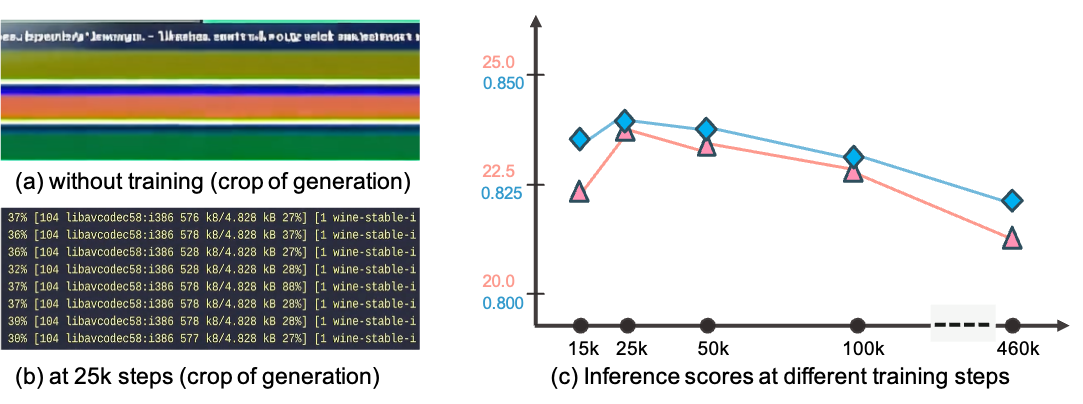
\includegraphics[width=\linewidth]{assets/train_metrics_curve10.png}
  \caption{(a--b) Qualitative generations before and after CLIGen training; (c) CLIGen (Clean) \PSNR/\SSIM~plateau around 25k training steps.}
  \label{fig:cligen-long-train}
  \vspace{-0.8em}
\end{wrapfigure}

Panels (a--b) illustrate the effect of training on CLIGen data.
Without CLIGen fine-tuning, Wan2.1 produces garbled terminal outputs (a).
After 25k steps, the model generates readable text with consistent formatting and color cues (b).

Figure~\ref{fig:cligen-long-train} plots the corresponding \PSNR/\SSIM~curves and indicates a clear efficiency ceiling.
These metrics peak around 25k steps and show little improvement with further training up to 460k steps.
Extended training can even slightly degrade performance.
One plausible explanation is that most learnable structured patterns are acquired early, and further gains require higher-quality, better-paced, or more informative supervision.

\exptitle[\cligenGeneralLogo]{3}{Literal captions drive rendering accuracy}



Caption specificity has a strong effect on terminal rendering quality.
As shown in Table~\ref{tab:cligen-captions}, detailed, literal descriptions improve reconstruction fidelity.
\PSNR increases from 21.90~dB (semantic) to 26.89~dB (detailed), a gain of nearly 5~dB, compared to less specific, high-level semantic descriptions.

The three caption tiers correspond to the same underlying terminal sequence but differ in length and granularity.
\textbf{Semantic} captions (average 55 words) provide high-level summaries (e.g., ``a terminal session generates three cat images'').
\textbf{Regular} captions (average 52 words) include key commands and outputs (e.g., \texttt{ai -i 3 a cute cat}, status messages).
\textbf{Detailed} captions (average 76 words) transcribe screen content more exhaustively, including exact text, colors, and formatting.

\begin{wraptable}{r}{0.42\linewidth}
  \vspace{-1.8em}
  \captionsetup{type=table,width=\linewidth}
  \centering
  \small
  \rowcolors{2}{metablue!8}{white}
  \caption{Caption styles versus TI2V fidelity.}
  \label{tab:cligen-captions}
  \setlength{\tabcolsep}{5pt}
  \begin{tabularx}{\linewidth}{l >{\centering\arraybackslash}X >{\centering\arraybackslash}X >{\centering\arraybackslash}X}
    \toprule
    \rowcolor{metablue!16} \textbf{Prompt style} & \textbf{\PSNR} & \textbf{\SSIM} & \textbf{Avg. words} \\
    Semantic & 21.90 & 0.813 & 55 \\
    Regular & 23.63 & 0.843 & 52 \\
    Detailed & \textbf{26.89} & \textbf{0.867} & \textbf{76} \\
    \bottomrule
  \end{tabularx}
  \vspace{-1.5em}
\end{wraptable}
This progression helps explain why literal descriptions are particularly effective for terminal rendering.
Unlike natural images, which are dominated by global style patterns, terminal frames are governed primarily by text placement.
% Detailed captions act as scaffolding by specifying which tokens appear where, enabling precise text-to-pixel alignment.
% This matches the observed gains as caption specificity increases.
Detailed captions act as scaffolding—explicitly specifying which tokens appear where—thereby enabling precise text-to-pixel alignment.



\exptitle[\cligenCleanLogo]{4}{Neural computers achieve accurate character-level text generation}

\begin{wraptable}{r}{0.42\linewidth}
  \vspace{-0.8em}
  \captionsetup{type=table,width=\linewidth}
  \centering
  \small
  \rowcolors{2}{metablue!8}{white}
  \caption{OCR accuracy versus training.}
  \label{tab:cligen-ocr}
  \setlength{\tabcolsep}{7pt}
  \begin{tabularx}{\linewidth}{l >{\centering\arraybackslash}X >{\centering\arraybackslash}X}
    \toprule
    \rowcolor{metablue!16} \textbf{Steps (k)} & \textbf{Char. acc.} & \textbf{Exact line} \\
    0  & 0.03 & 0.01 \\
    10 & 0.18\,$\color{green!60!black}{\uparrow}_{0.15}$ & 0.05\,$\color{green!60!black}{\uparrow}_{0.04}$ \\
    20 & 0.33\,$\color{green!60!black}{\uparrow}_{0.30}$ & 0.12\,$\color{green!60!black}{\uparrow}_{0.11}$ \\
    30 & 0.41\,$\color{green!60!black}{\uparrow}_{0.38}$ & 0.18\,$\color{green!60!black}{\uparrow}_{0.17}$ \\
    40 & 0.52\,$\color{green!60!black}{\uparrow}_{0.49}$ & 0.26\,$\color{green!60!black}{\uparrow}_{0.25}$ \\
    50 & 0.52\,$\color{green!60!black}{\uparrow}_{0.49}$ & 0.27\,$\color{green!60!black}{\uparrow}_{0.26}$ \\
    60 & \textbf{0.54}\,$\color{green!60!black}{\uparrow}_{0.51}$ & \textbf{0.31}\,$\color{green!60!black}{\uparrow}_{0.30}$ \\
    \bottomrule
  \end{tabularx}
  \vspace{-0.8em}
\end{wraptable}

Beyond PSNR and SSIM, character-level accuracy is a more direct metric for terminal rendering.
Character-level accuracy requires explicit pixel-to-text correspondence.
For CLIGen (Clean), we apply Tesseract to five uniformly sampled (ground-truth, generated) frame pairs per video and normalize whitespace.
We then compute two metrics (full protocol in Appendix~\ref{appendix:pipeline}).
Character accuracy uses the Levenshtein distance between concatenated ground-truth and generated texts.
Exact-line accuracy measures the fraction of ground-truth lines whose normalized content exactly matches the prediction at the same line index.

Table~\ref{tab:cligen-ocr} shows that our models achieve substantial text rendering accuracy under this protocol.
Character accuracy increases from 0.03 at initialization to 0.54 at 60k steps, with exact-line matches reaching 0.31 (0.26 by 40k).
Most gains occur within the first 40k steps, followed by smaller refinements thereafter.
These OCR-based metrics capture properties beyond perceptual similarity. 
Accurately generating terminal characters requires modeling text structure, font rendering, and spatial relationships.
These are core competencies for interactive neural computer systems.
This level of character-level precision is a step toward usable, not just plausible, terminal interfaces.



\exptitle[\cligenCleanLogo]{5}{Does this NC instantiation show native CLI reasoning?}

\providecommand{\wanicon}{\raisebox{-0.25ex}{
\includegraphics[height=1.00em]{assets/wan_icon.png}}}
\providecommand{\veoicon}{\raisebox{-0.25ex}{
\includegraphics[height=1.00em]{assets/veo_ICON.png}}}
\providecommand{\soraicon}{\raisebox{-0.25ex}{
\includegraphics[height=1.00em]{assets/sora_icon.png}}}
\begin{wraptable}{r}{0.50\linewidth}
  \vspace{-1.0em}
  \captionsetup{type=table,width=\linewidth}
  \centering
  \small
  \rowcolors{2}{metablue!8}{white}
  \caption{Arithmetic probe accuracy (100 problems sampled from a 1{,}000-problem held-out pool).}
  \label{tab:cligen-arith}
  \setlength{\tabcolsep}{8pt}
  \begin{tabularx}{\linewidth}{l >{\centering\arraybackslash}X}
    \toprule
    \rowcolor{metablue!16} \textbf{Model} & \textbf{Accuracy} \\
    \wanicon\;Wan2.1 & 0\% \\
    \cligenCleanLogo{}\;\nccligen{} & 4\% \\
    \veoicon\;Veo3.1 & 2\% \\
    \soraicon\;Sora2 & \textbf{71}\% \\
    % \cligenCleanLogo{}\;\nccligen{} + reprompt & \textbf{83\%} \\
    \bottomrule
  \end{tabularx}
   \vspace{-1.0em}
\end{wraptable}
We also probe symbolic computation with CLI arithmetic tasks.
These tasks are a sharp stress test for symbolic reliability: humans answer them instantly, yet current NC instantiations often fail on seemingly simple symbolic operations.

Our arithmetic probe presents basic mathematical operations through terminal interactions.
We reserve a held-out pool of 1{,}000 math problems and randomly sample 100 problems as the final evaluation set.
Table~\ref{tab:cligen-arith} shows that current video models, including this NC instantiation, struggle on these symbolic tasks.
Wan2.1 achieves 0\% accuracy, our \nccligen{} model reaches 4\%, and Veo3.1 manages 2\%—all far below human-level performance on these fundamental tasks.
%
These results contrast with common claims of strong symbolic reasoning in current video models.
Sora2's 71\% accuracy is a notable outlier and may reflect system-level advantages or additional training beyond our current setup.
Overall, native symbolic reasoning remains an open challenge for current video-based NC~instantiations.




The poor arithmetic-probe performance in Table~\ref{tab:cligen-arith} raises a key question.
Does this prototype require specialized reinforcement learning to achieve reliable symbolic computation, or can stronger conditioning substantially narrow this gap?
% Sora2's 71\% accuracy suggests several possible explanations, which we examine systematically in Table~\ref{tab:sora-leads}. 


\exptitle[\cligenCleanLogo]{6}{Does this NC instantiation require RL for symbolic probes?}
\begin{wrapfigure}{r}{0.49\linewidth}
  \vspace{-1.8em}
  \centering
  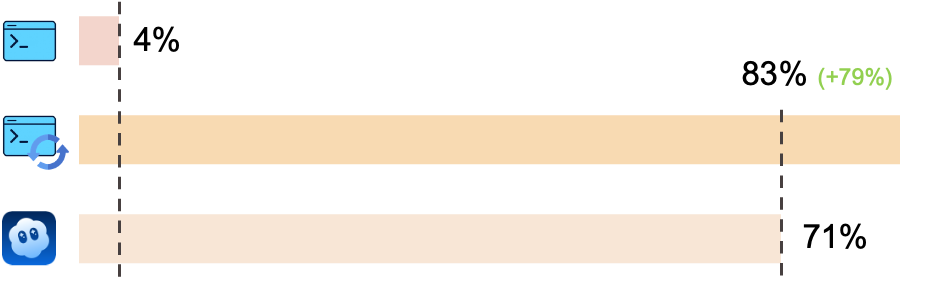
\includegraphics[width=\linewidth]{assets/cligen_exp6v3.png}
  \caption{Reprompting boosts performance to 83\%.}
  \label{fig:cligen-exp6}
  \vspace{-1.0em}
\end{wrapfigure}

As shown in Figure~\ref{fig:cligen-exp6}, \nccligen{} accuracy on CLIGen (Clean) arithmetic tasks rises from 4\% to 83\% under reprompting.
This suggests that system-level conditioning can be an effective first lever for improving performance on symbolic probes.
It is complementary to (rather than strictly requiring) RL-based training pipelines.
%
More generally, the success of reprompting highlights how sensitive symbolic-probe outcomes are to the conditioning interface.
Much of the apparent ``reasoning'' gain can come from better specification and instruction-following rather than new native computation.
For the arithmetic subset, we include the correct answer explicitly in roughly half of the training captions to encourage reliable rendering of the output string.
Because reprompting can similarly provide stronger hints (or even outsource computation to an external text system), we interpret the gain primarily as evidence of steerability.
It also shows faithful rendering of conditioned symbolic content.
We do not treat it as a clean demonstration that the NC backbone performs arithmetic internally.




\begin{table}[h]
  \captionsetup{type=table,width=\linewidth}
  \centering
  \small
  \rowcolors{2}{metablue!8}{white}
\caption{Hypotheses for Sora2's advantage.}
 \vspace{-4pt}
  \label{tab:sora-leads}
  \setlength{\tabcolsep}{6pt}
  \begin{tabularx}{\linewidth}{l X}
    \toprule
    \rowcolor{metablue!16} \textbf{Factor} & \textbf{Implication} \\
    \tikz[baseline=-0.35ex]{\node[fill=metablue, text=white, circle, inner sep=1.2pt, font=\scriptsize\bfseries] {1};} Stronger base + similar data & Higher intrinsic arithmetic; symbolic capability may be baked in \\
    \tikz[baseline=-0.35ex]{\node[fill=orange!85!red, text=white, circle, inner sep=1.2pt, font=\scriptsize\bfseries] {2};} Additional RL training & Reward shaping teaches math beyond diffusion; could transfer to CLI \\
    \tikz[baseline=-0.35ex]{\node[fill=teal!70!black, text=white, circle, inner sep=1.2pt, font=\scriptsize\bfseries] {3};} System-level reprompt/recaption & LLM computes answers; strong conditioning drives generation \\
    \bottomrule
  \end{tabularx}
\end{table}

The evidence supports system-level conditioning as a practical path forward for this NC instantiation.
Among the three hypotheses for improving arithmetic-probe performance—stronger base models, reinforcement learning, or enhanced conditioning—our results most strongly favor the third approach.
The gain from reprompting (4\%$\rightarrow$83\%), achieved without modifying the underlying NC backbone, is substantial.
It shows that measured ``reasoning'' on these probes is highly sensitive to specification and conditioning.
We therefore do not treat it as direct evidence of native arithmetic inside the NC backbone.

In our setting, strategic conditioning yields larger symbolic-probe gains than the RL pipeline we tested.
Evaluations should therefore distinguish native computation from conditioning-assisted performance when assessing reasoning capabilities in current video-based NC instantiations.






\subsubsection{Visualizations}

\noindent\textbf{(1) \cligenGeneralData{} visualizations.}
Qualitative samples highlight the breadth of real-world terminal dynamics captured in CLIGen (General): ANSI escape sequences that repaint regions with changing foreground/background colors, incremental command entry with syntax highlighting and cursor edits, classic shell prompts and system outputs, long-running jobs with rapidly scrolling and color-coded package logs, full-screen TUIs such as partition editors, and progress dashboards with updating bars, counts, and ETAs.
These traces emphasize that ``looking correct'' requires maintaining terminal geometry, palette transitions, and cursor state frame-by-frame.

\noindent\textbf{(2) \cligenCleanData{} REPL visualizations.}
In contrast to open-world traces, CLIGen (Clean) REPL samples are scripted and temporally well-paced (Figures~\ref{fig:cligen-clean-viz-a}--\ref{fig:cligen-clean-viz-d}; additional examples are in Appendix~\ref{appendix:cligen-samples}).
Each sample includes an explicit action trace (e.g., \texttt{Sleep}, \texttt{Type}, \texttt{Enter}, arrow keys, \texttt{Hide}) alongside rendered terminal frames, making the action-to-pixel link visually unambiguous.
The key insight is that these scripted traces isolate rendering-and-control errors from semantic ambiguity: with explicit actions, failures are dominated by low-level mechanics (cursor placement, character edits, monospace alignment, line breaks, temporal consistency).

\noindent\textbf{(3) \cligenCleanData{} math visualizations.}
Figures~\ref{fig:cligen-clean-math-comp-a}--\ref{fig:cligen-clean-math-comp-c} compare math REPL rollouts, and Figures~\ref{fig:cligen-clean-math-rep-a}--\ref{fig:cligen-clean-math-rep-c} show reprompting cases.
Together they highlight why arithmetic probes should separate native computation from answer-conditioned rendering.
All full-resolution pages are in Appendix~\ref{appendix:vis}; below we keep clickable thumbnails at the original location for quick navigation.

\newcommand{\CliThumbPageHeader}[1]{%
  \par\noindent\makebox[\linewidth][c]{%
    \fcolorbox{metablue!45}{metablue!5}{%
      \begin{minipage}{0.94\linewidth}
        \centering
        \vspace{0.22em}
        {\large\bfseries #1}\par
        \vspace{0.1em}
        {\scriptsize\textsf{\color{metablue!85!black}Click any thumbnail to jump to its full-resolution page in Appendix}}\par
        \vspace{0.18em}
      \end{minipage}
    }%
  }\par\vspace{0.58em}%
}
\newcommand{\CliThumbPageHeaderSimple}[1]{%
  \par\noindent\makebox[\linewidth][c]{%
    \fcolorbox{metablue!45}{metablue!5}{%
      \begin{minipage}{0.94\linewidth}
        \centering
        \vspace{0.22em}
        {\large\bfseries #1}\par
        \vspace{0.16em}
      \end{minipage}
    }%
  }\par\vspace{0.58em}%
}
\newcommand{\CliThumbPageHeaderPlain}[1]{%
  {\par\noindent\centering\Large\bfseries #1\par}
  {\par\noindent\centering%
    \begin{tcolorbox}[
      enhanced,
      boxrule=0.85pt,
      colframe=orange!80!black,
      colback=yellow!14,
      arc=5.5pt,
      left=6pt,right=6pt,top=2.5pt,bottom=2.5pt,
      width=0.78\linewidth
    ]
      \centering\small\bfseries\sffamily\color{orange!85!black}
      Click any thumbnail to jump to its full-resolution page in Appendix
    \end{tcolorbox}\par
  }
  \vspace{0.26em}%
}
\newcommand{\CliThumbPageFrame}{%
  \begin{tikzpicture}[remember picture,overlay]
    \draw[
      draw=black,
      line width=1.9pt,
      rounded corners=14pt
    ]
      ([xshift=0.48cm,yshift=-0.48cm]current page.north west)
      rectangle
      ([xshift=-0.48cm,yshift=0.48cm]current page.south east);
  \end{tikzpicture}%
}
\newcommand{\CliThumbCard}[4]{%
  \par\noindent\makebox[\linewidth][c]{%
    \hyperref[#1]{%
      \begin{tikzpicture}
        \node[inner sep=0pt] (img) {\includegraphics[width=#4\linewidth,keepaspectratio]{#2}};
        \node[
          anchor=south east,
          xshift=-0.38em,
          yshift=0.26em,
          fill=white,
          fill opacity=0.93,
          text opacity=1,
          draw=metablue!50,
          rounded corners=1.5pt,
          inner xsep=0.45em,
          inner ysep=0.2em,
          minimum width=8.4em,
          align=center,
          font=\scriptsize\bfseries,
          text=metablue!90!black
        ] at (img.south east) {#3};
      \end{tikzpicture}%
    }%
  }\par\vspace{0.28em}%
}
\newcommand{\CliThumb}[4]{\CliThumbCard{#1}{#2}{#3}{#4}}

\clearpage
\newgeometry{top=0.9cm,bottom=1.35cm,left=0.9cm,right=0.9cm,includefoot,footskip=18pt}
\thispagestyle{plain}
\hypertarget{main-cligen-vis-thumbs}{}
\hypertarget{main-cligen-vis-thumbs-p1}{}
\hypertarget{main-cligen-vis-thumbs-p2}{}
\CliThumbPageFrame
\CliThumbPageHeaderPlain{CLIGen Visualization Thumbnails}
\noindent\begin{tabular}{@{}p{0.495\linewidth}!{\color{metablue!55}\vrule width 0.8pt}p{0.495\linewidth}@{}}
\begin{minipage}[t]{\linewidth}
  \vspace*{0pt}
  \centering
  {\small\bfseries \cligenGeneralLogo{}\ CLIGen (General) Visualizations}\par
  \vspace{0.14em}
  \CliThumb{fig:cligen-general-viz-1}{assets/cligen_general_1.pdf}{\cligenGeneralLogo{}\ Samples A}{0.72}
  \CliThumb{fig:cligen-general-viz-2}{assets/cligen_general_2.pdf}{\cligenGeneralLogo{}\ Samples B}{0.72}
  \CliThumb{fig:cligen-general-viz-3}{assets/cligen_general_3.pdf}{\cligenGeneralLogo{}\ Samples C}{0.72}
\end{minipage}
&
\begin{minipage}[t]{\linewidth}
  \vspace*{0pt}
  \centering
  {\small\bfseries \cligenCleanLogo{}\ CLIGen (Clean) Visualizations}\par
  \vspace{0.14em}
  \CliThumb{fig:cligen-clean-viz-a}{assets/cligen_clean_1.pdf}{\cligenCleanLogo{}\ Samples A}{0.97}
  \CliThumb{fig:cligen-clean-viz-b}{assets/cligen_clean_2.pdf}{\cligenCleanLogo{}\ Samples B}{0.97}
  \CliThumb{fig:cligen-clean-viz-c}{assets/cligen_clean_3.pdf}{\cligenCleanLogo{}\ Samples C}{0.97}
  \CliThumb{fig:cligen-clean-viz-d}{assets/cligen_clean_4.pdf}{\cligenCleanLogo{}\ Samples D}{0.97}
\end{minipage}
\end{tabular}
\restoregeometry
\par\justifying

\clearpage
\newgeometry{top=0.9cm,bottom=1.35cm,left=0.9cm,right=0.9cm,includefoot,footskip=18pt}
\thispagestyle{plain}
\hypertarget{main-cligen-vis-thumbs-p3}{}
\hypertarget{main-cligen-vis-thumbs-p4}{}
\CliThumbPageFrame
\CliThumbPageHeaderPlain{CLIGen Visualization Thumbnails}
\noindent\begin{tabular}{@{}p{0.495\linewidth}!{\color{metablue!55}\vrule width 0.8pt}p{0.495\linewidth}@{}}
\begin{minipage}[t]{\linewidth}
  \vspace*{0pt}
  \centering
  {\small\bfseries \cligenCleanLogo{}\ CLIGen (Clean) Math Comparison}\par
  \vspace{0.14em}
  \CliThumb{fig:cligen-clean-math-comp-a}{assets/cligen_math_comp1.pdf}{\cligenCleanLogo{}\ Samples A}{0.76}
  \CliThumb{fig:cligen-clean-math-comp-b}{assets/cligen_math_comp2.pdf}{\cligenCleanLogo{}\ Samples B}{0.76}
  \CliThumb{fig:cligen-clean-math-comp-c}{assets/cligen_math_comp3.pdf}{\cligenCleanLogo{}\ Samples C}{0.76}
\end{minipage}
&
\begin{minipage}[t]{\linewidth}
  \vspace*{0pt}
  \centering
  {\small\bfseries \cligenCleanLogo{}\ CLIGen (Clean) Math Reprompting}\par
  \vspace{0.14em}
  \CliThumb{fig:cligen-clean-math-rep-a}{assets/cligen_math_rep1.pdf}{\cligenCleanLogo{}\ Samples A}{0.98}
  \CliThumb{fig:cligen-clean-math-rep-b}{assets/cligen_math_rep2.pdf}{\cligenCleanLogo{}\ Samples B}{0.98}
  \CliThumb{fig:cligen-clean-math-rep-c}{assets/cligen_math_rep3.pdf}{\cligenCleanLogo{}\ Samples C}{0.98}
\end{minipage}
\end{tabular}
\restoregeometry
\par\justifying


\par\justifying

\newpage
\subsection{\guiworldLogo{}\,The GUI World Models}
\label{section:impl-guiworld}
\justifying
We also instantiate the NC abstraction in interactive desktop environments with \ncguiworld{}.
In this setting, fine-grained action control is essential: GUI interaction requires precise cursor tracking, timely click feedback, and robustness to rapidly changing interface states.
We model each interaction as a synchronized sequence of RGB frames $x_t$ and input events $u_t$ (mouse and keyboard).
The latent video state maintains interface context across frames, while temporally aligned action inputs provide control signals designed to preserve pixel-level correspondence between user actions and visual changes.


\subsubsection{Data pipeline}
\label{section:impl-guiworld-data-pipeline}
\begin{wraptable}{r}{0.48\linewidth}
  \vspace{-1.7em}
  \captionsetup{type=table,width=\linewidth}
  \centering
  \small
  \rowcolors{2}{metablue!8}{white}
  \caption{Cursor/action statistics.}
  \label{tab:gui-stats}
  \setlength{\tabcolsep}{7pt}
  \begin{tabularx}{\linewidth}{l >{\centering\arraybackslash}X >{\centering\arraybackslash}X}
    \toprule
    \rowcolor{metablue!16}\textbf{Split} & \textbf{Avg. cursor speed (px/frame)} & \textbf{Actions / sec} \\
    Random Slow & 1.51 & 1.58 \\
    Random Fast & 195.15 & 4.18 \\
    CUA (supervised) & 3.79 & 0.10 \\
    \bottomrule
  \end{tabularx}
  \vspace{-0.8em}
\end{wraptable}

% We collect GUI data at 15~FPS with synchronized cursor and keyboard logs. 
The dataset includes two styles of random interaction: ``Random Slow'' and ``Random Fast'', plus a smaller set of supervised trajectories collected by Claude CUA~\citep{claudeComputerTool}.
Random Slow (approximately 1{,}000 hours) contains longer pauses, idle gaps, and deliberate cursor movements, which can expose cursor drift after extended inactivity.
Random Fast (approximately 400 hours) features denser cursor motion and typing bursts, stressing acceleration dynamics and hover timing.
%
The supervised trajectories are approximately 110 hours. 
These goal-directed traces provide higher-signal action--response pairs without overwhelming the exploration data.
Table~\ref{tab:gui-stats} summarizes cursor and action statistics across splits; in the collected CUA trajectories, action density is lower due to latency introduced by Claude’s tool API between successive steps.


All GUI data is collected inside an Ubuntu~22.04 container running XFCE4 (Arc-Dark theme, Papirus icons) on a fixed 1024$\times$768 virtual display at 15~FPS.
We render the display with Xvfb and interact through a VNC/noVNC stack.
The desktop pins a small open-source app set to launchers.
It includes Firefox ESR, GIMP, VLC, VS~Code, Calculator, Terminal, the file manager, and the Mahjongg game, matching the environment shown in our recordings.
Screen capture uses \texttt{mss} and \texttt{ffmpeg} with cursor overlays, and actions are replayed and logged via \texttt{xdotool}.
%
We keep the recorded discontinuities and interface latency intact rather than smoothing them.
In dataset packaging, we store both raw-action and meta-action views for modeling.
This lets us train either the raw-action or meta-action encoder under the same loss stack\footnote{Conversion details and alignment quality appear in Appendix~\ref{appendix:gui-actions}.}.







\subsubsection{Model architecture}


The GUIWorld architecture builds on the Wan2.1~\citep{wan2025wan} by incorporating explicit action-conditioning modules.
The central challenge is to align time-stamped user actions with generated frames and inject this information at the appropriate depth within the transformer.


Action features are encoded on-the-fly from frame-aligned mouse and keyboard signals (Section~\ref{section:impl-guiworld-data-pipeline}).
We aggregate them into latent-aligned embeddings that summarize recent action history at each diffusion step.
%
We evaluate two action encoders.
The \emph{raw-action encoder} (v1) preserves fine-grained mouse/keyboard event streams.
The \emph{meta-action encoder} (v2) abstracts interactions into coarse API-style categories (clicks, drags, scrolls, typing, shortcuts).
Both encoders use the same temporal alignment and are evaluated as separate ablations.
In our experiments, their differences in rendering fidelity and control behavior are modest\footnote{Appendix Table~\ref{tab:action-encoder-comparison} summarizes the representational differences.}.


We inject action embeddings into the diffusion backbone in four ways (Figure~\ref{fig:action-injection}).
We study \texttt{external}, \texttt{contextual}, \texttt{residual}, and \texttt{internal} conditioning.
For the injection-scheme ablation, all four modes share the same meta-action encoder and temporal alignment.
They differ only in where the latent action features interact with the video latents and transformer blocks.
We compare raw-action vs.\ meta-action encoders separately in Table~\ref{tab:gui-encoding-ablation}.



\noindent\textbf{External conditioning.}
In the \texttt{external} mode, action information modulates the latent video sequence before the diffusion transformer.
Action features are applied as a pre-conditioning step at the model input, without introducing explicit action tokens or cross-attention inside the diffusion backbone.
As a result, action information enters only through the modified input latents; the diffusion backbone never attends directly to action tokens, so any action signal must be carried implicitly in $z'_{1:T}$.

Formally, given VAE latents $z_{1:T}$ and temporally aligned action features $u_{1:T}$, an external action module applies a small stack of temporal self-attention and action cross-attention layers.
This produces a residual update $\Delta z_{1:T}(u_{1:T})$.
The modified latents are
\[
  z'_{1:T} = z_{1:T} + \Delta z_{1:T}(u_{1:T}),
\]
and the diffusion transformer operates solely on $z'_{1:T}$.
The diffusion backbone remains unchanged, and action features are not exposed as explicit tokens within the transformer.



\begin{figure}[t]
  \centering
  \DeclareRobustCommand{\modeExt}{\tikz[baseline=-0.2em]{\node[fill=red!70, circle, inner sep=1.6pt, text=white, font=\scriptsize]{1};}}
  \DeclareRobustCommand{\modeCtx}{\tikz[baseline=-0.2em]{\node[fill=blue!70, circle, inner sep=1.6pt, text=white, font=\scriptsize]{2};}}
  \DeclareRobustCommand{\modeRes}{\tikz[baseline=-0.2em]{\node[fill=orange!80, circle, inner sep=1.6pt, text=white, font=\scriptsize]{3};}}
  \DeclareRobustCommand{\modeInt}{\tikz[baseline=-0.2em]{\node[fill=teal!70, circle, inner sep=1.6pt, text=white, font=\scriptsize]{4};}}
  
\includegraphics[width=\linewidth]{assets/action_injection4.pdf}
  \vspace{0.2em}
  \small
  \setlength{\tabcolsep}{4pt}
  \renewcommand{\arraystretch}{1.05}
  \begin{tabularx}{\linewidth}{@{}l >{\raggedright\arraybackslash}p{0.30\linewidth} X@{}}
    \toprule
    \textbf{Mode} & \textbf{Injection point} & \textbf{Notes} \\
    \modeExt\ \texttt{external} & Conditioned VAE input & Actions are injected as an external conditioning stream that modulates the backbone without sharing the main token sequence. \\
    \modeCtx\ \texttt{contextual} & Concat frames, actions & Video and action tokens share one sequence with a lag-aware temporal attention mask, enabling mid-level fusion. \\
    \modeRes\ \texttt{residual} & Hidden state with action delta & Actions are added through residual-style modulation branches, acting as a strong but more indirect baseline. \\
    \modeInt\ \texttt{internal} & After cross-attn, before FFN & Actions enter through dedicated cross-attention inside the transformer blocks, fusing near the backbone core. \\
    \bottomrule
  \end{tabularx}
  \vspace{0.1em}
  \captionsetup{justification=raggedright,singlelinecheck=false}
\caption{\textbf{Four modes for injecting GUI actions into the diffusion transformer.}
\modeExt{} modulates VAE latents before the transformer;
\modeCtx{} adds action tokens alongside visual tokens;
\modeRes{} applies block-wise residual updates; and
\modeInt{} inserts an action cross-attention module inside transformer blocks.}

  \label{fig:action-injection}
\end{figure}

\noindent\textbf{Contextual conditioning.}
In the \texttt{contextual} mode, actions are represented as additional tokens and integrated directly into the transformer’s self-attention.
Similar token-based action representations have been explored in prior world models, including Gato~\citep{reed2022generalist} and World and Human Action Models~\citep{kanervisto2025world}.

The meta-action encoder produces latent-aligned action tokens $A \in \mathbb{R}^{L_a \times D}$.
We concatenate them with visual tokens $V \in \mathbb{R}^{L_v \times D}$ to form a joint sequence $[V; A]$.
Each transformer block applies self-attention over this combined sequence using a structured temporal mask (Appendix Figure~\ref{fig:contextual-mask}).
The mask enforces causal alignment: each frame token attends only to actions within a short past window, and each action token attends only to frames after a fixed temporal lag.
Through this masked joint attention, \texttt{contextual} conditioning fuses action and visual information within the transformer blocks.


\noindent\textbf{Residual conditioning.}
In the \texttt{residual} mode, the transformer block structure remains unchanged.
A lightweight action module attaches to a subset of layers as an external residual branch.
This follows the \texttt{residual} conditioning paradigm introduced by ControlNet~\citep{zhang2023adding}, while remaining modular and additive to the base diffusion backbone.

At each selected layer $l$, the transformer applies its standard sequence of self-attention, text or reference cross-attention, and feed-forward operations to produce hidden states $h^{(l)}$.
A separate action module then takes $h^{(l)}$ together with a local temporal window of latent action features and mouse trajectories.
It outputs a residual update $\Delta h^{(l)}(a,\text{mouse})$.
The updated hidden states are given by
\[
  \tilde{h}^{(l)} = h^{(l)} + \Delta h^{(l)}(a,\text{mouse}),
\]
which are passed to the subsequent transformer block.
In this formulation, \texttt{residual} conditioning injects action information through block-external residual branches.
It does not modify the internal computations of the transformer blocks themselves.


\noindent\textbf{Internal conditioning.}
In the \texttt{internal} mode, action conditioning is incorporated directly within the transformer blocks.
Related multi-stream world models have explored similar designs, including Matrix-Game-2~\citep{he2025matrix}.
Each selected block augments the standard attention stack with an additional action cross-attention sub-layer.
Specifically, the block applies self-attention, followed by cross-attention over text and reference features, and then a dedicated action cross-attention layer.
Keys and values are derived from latent action features (and, optionally, mouse inputs).

Given block input $h$, text or reference context $c$, and action latents $a$, the internal block computes
\[
  h' = \mathrm{FFN}\Big(
    h + \mathrm{CA}_{\text{text}}\big(\mathrm{SA}(h), c\big)
      + \mathrm{CA}_{\text{action}}(h, a)
  \Big),
\]
where $\mathrm{SA}$ denotes self-attention and $\mathrm{CA}_{\text{text}}$ and $\mathrm{CA}_{\text{action}}$ denote the text and action cross-attention modules applied in sequence.
As illustrated in Figure~\ref{fig:action-injection}, action features are injected directly into the block’s cross-attention stage.

In contrast to \texttt{residual} conditioning, \texttt{internal} conditioning integrates action information through a block-internal attention mechanism rather than an external residual branch.
This design mirrors the multi-stream injection strategy used in Matrix-Game-2~\citep{he2025matrix} and yields the best SSIM/FVD trade-off for fine-grained GUI interaction in our ablations.
In this setting, precise temporal alignment and spatial locality are critical.
Each conditioning mode (\texttt{external}, \texttt{contextual}, \texttt{residual}, and \texttt{internal}) is trained as a separate ablation, and no combinations are used.


\subsubsection{Implementation Details}
We train one model per injection mode (\texttt{external}, \texttt{contextual}, \texttt{residual}, \texttt{internal}), keeping the backbone and all non-action components fixed.
Each run lasts about 64k steps.
We tune only the action encoder and learning-rate schedule.
Training optimizes the diffusion loss together with a small temporal contrastive loss that aligns frame features with action and mouse embeddings (Appendix~\ref{appendix:gui-actions}).
Runs use 64 GPUs for about 15 days, totaling about 23k GPU-hours per full pass.

Preprocessing is implemented in the data loader in two stages.
First, we normalize each recording to a fixed resolution and frame rate.
This produces tensors for RGB video, per-frame cursor coordinates, and mouse/keyboard event traces (in both raw-action and meta-action views).
Second, we render an SVG cursor at each logged position to produce per-frame masks and cursor-only reference frames.
The first reference frame contains the full desktop with a unit mask.
Later references paste only the cursor over a neutral background, with a mask restricted to arrow pixels.
After VAE encoding, these references become latent slots that pin down the static GUI layout at $t{=}0$.
For $t{>}0$, they supervise only a small patch around the cursor and leave the rest of the frame unconstrained.
We drop clips without valid cursor or action traces to keep~supervision~consistent.

\subsubsection{Evaluation setup}
Our ablations target three capabilities: global fidelity, post-action responsiveness, and cursor-control precision.
We use the \FVD/\LPIPS/\SSIM~suite as the core metrics.
We also add action-driven metrics that focus on post-interaction frames after clicks, scrolls, and key/type events.
For example, we compute \SSIM/\LPIPS~averaged over the $k$ frames after each logged action, and action-driven \FVD~on post-action clips.
Ablations vary conditioning design and action encoding to measure how these choices affect perceptual quality and responsiveness when rolled out against ground-truth interfaces\footnote{Full metric definitions and implementation details are provided in Appendix~\ref{appendix:gui-metrics}.}.


\exptitle[\guiworldLogo]{7}{Data quality dominates performance}



Interactive GUI modeling shows that data quality matters more than dataset size for action-driven performance.
We compare slow exploration, fast interaction, and supervised trajectories under \texttt{contextual} conditioning.
This isolates which behaviors best support neural computer training.




\begin{wraptable}{r}{0.48\linewidth}
  \vspace{-0.1em}
  \captionsetup{type=table,width=\linewidth}
  \centering
  \small
  \rowcolors{2}{metablue!8}{white}
  \caption{Overall performance across data sources.}
  \label{tab:gui-data-quality}
  \setlength{\tabcolsep}{7pt}
  \begin{tabularx}{\linewidth}{l >{\centering\arraybackslash}X >{\centering\arraybackslash}X >{\centering\arraybackslash}X}
    \toprule
    \rowcolor{metablue!16}\textbf{Split} & \textbf{FVD$_\text{all}$} & \textbf{SSIM$_\text{all}$} & \textbf{LPIPS$_\text{all}$} \\
    Untrained baseline & 149.61 & 0.496 & 0.605 \\
    Random Fast (train) & 48.17 & 0.695 & 0.483 \\
    Random Slow (train) & 20.37 & 0.830 & 0.237 \\
    Claude CUA (train) & 14.72 & 0.885 & 0.144 \\
    \bottomrule
  \end{tabularx}
  \vspace{-1.8em}
\end{wraptable}

Despite approximately 1{,}400 hours of random exploration across the slow and fast settings, these datasets are noisy.
They are comparatively sample-inefficient for learning stable action--response mappings.
They substantially improve global perceptual metrics over a baseline (Table~\ref{tab:gui-data-quality}).
However, high-frequency cursor jitter and irregular, non-goal-directed action bursts make consistent control difficult under dense, stochastic input streams.

In contrast, the substantially smaller high-quality dataset (110 hours from Claude CUA) yields markedly stronger performance across all metrics.
Goal-directed trajectories provide clearer action semantics and more predictable state transitions.
This enables robust action conditioning even with limited data volume.
These results indicate that neural computer development should prioritize curated, purposeful interactions over large-scale passive data collection.



\exptitle[\guiworldLogo]{8}{Precise cursor control requires explicit visual supervision}

\begin{figure}[h]
  \centering
  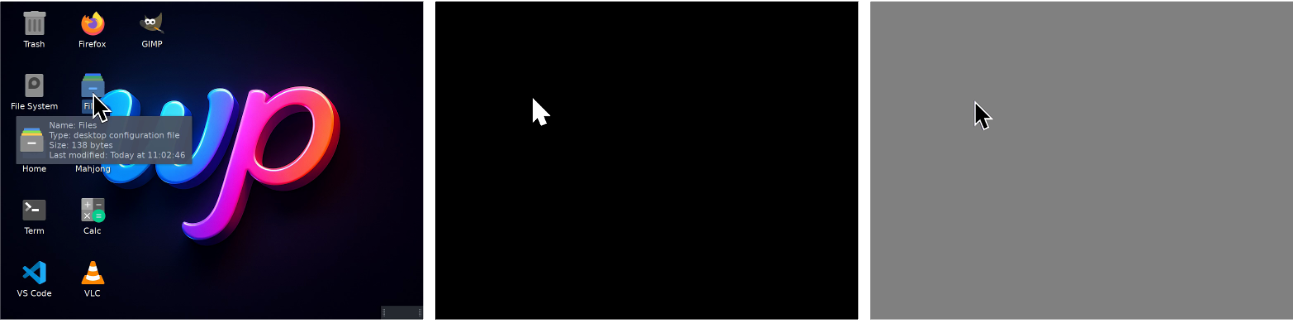
\includegraphics[width=\linewidth]{assets/ref2.png}
\caption{\textbf{Cursor references in GUIWorld.}
\textbf{Left:} original desktop frames.
\textbf{Middle:} binary cursor masks.
\textbf{Right:} cursor-only reference frames rendered over a neutral background.}
  \label{fig:cursor-ref}
\end{figure}

\begin{wraptable}{r}{0.48\linewidth}
  \vspace{-1.0em}
  \captionsetup{type=table,width=\linewidth}
  \centering
  \small
  \rowcolors{2}{metablue!8}{white}
  \caption{Cursor conditioning losses versus accuracy.}
  \label{tab:cursor-loss}
  \setlength{\tabcolsep}{7pt}
  \begin{tabularx}{\linewidth}{l >{\centering\arraybackslash}X}
    \toprule
    \rowcolor{metablue!16}\textbf{Loss variant} & \textbf{Cursor accuracy} \\
    Position $(x,y)$ only & 8.7\% \\
    Position $(x,y)$ + Fourier & 13.5\% \\
    Position $(x,y)$ + SVG mask/ref & \textbf{98.7\%} \\
    \bottomrule
  \end{tabularx}
  \vspace{-0.8em}
\end{wraptable}

We examine whether the NC internalizes cursor dynamics.
A natural baseline is to condition on normalized cursor-coordinate sequences $\texttt{mouse\_trajectories}\subset[0,1]^{T\times 2}$ (details in Appendix~\ref{appendix:mouse-traj-normalization}). 
%
To strengthen this signal, we further encode the normalized trajectories using a Fourier mouse encoder.
We map coordinates to $[-1,1]^2$ and project them through a fixed Gaussian matrix to obtain random Fourier features.
A small MLP produces per-frame embeddings, which we aggregate into lag-aware windows aligned with the VAE stride.
The resulting latent action sequence conditions the action modules and participates in the temporal contrastive loss.

However, Table~\ref{tab:cursor-loss} shows that coordinate-based supervision remains insufficient for precise interaction.
Position-only supervision achieves 8.7\% accuracy, and even enhanced position features reach only 13.5\%.
This suggests that richer coordinate encodings alone do not resolve cursor drift and jitter.

Motivated by the importance of precise cursor placement, we introduce explicit visual cursor supervision.
We render an SVG cursor at each $(x_t,y_t)$ to produce per-frame cursor masks $m_t$ and cursor-only foregrounds $f_t$ (right panel of Figure~\ref{fig:cursor-ref}).
Following Figure~\ref{fig:cursor-ref}, we construct a reference stream.
The first frame contains the full desktop image, while subsequent frames contain only the cursor foreground over a neutral background, masked to the cursor region.
We encode both the video and reference streams with the shared VAE, yielding video latents $z_{1:T}$, reference latents $z^{\text{ref}}_{1:T}$, and mask tags $\tau_{1:T}$.
The diffusion transformer receives the concatenated tensor
\[
  \mathrm{concat}\bigl(z_{1:T},\,\tau_{1:T},\,z^{\text{ref}}_{1:T}\bigr),
\]
which anchors the static GUI layout at $t{=}0$ and provides localized supervision around the cursor for $t{>}0$.

Under this explicit visual conditioning, cursor accuracy improves to 98.7\%.
This suggests that neural computers benefit from learning the cursor state as a visual object rather than relying solely on abstract coordinates.
Explicit pixel-level supervision helps model cursor acceleration, hover states, and click feedback, which are essential for reliable GUI interaction.




\exptitle[\guiworldLogo]{9}{Action injection under different schemes}

\begin{table}[h]
  \centering
  \footnotesize
  \rowcolors{2}{metablue!8}{white}
  \caption{Action-driven metrics across injection schemes (15 frames after action).}
  \label{tab:gui-action-ssim}
  \setlength{\tabcolsep}{11pt}
  \begin{tabularx}{1\linewidth}{l >{\centering\arraybackslash}X >{\centering\arraybackslash}X >{\centering\arraybackslash}X}
    \toprule
    \rowcolor{metablue!16}
    \textbf{Mode} &
    \textbf{SSIM$_{+15}$} $\uparrow$ &
    \textbf{\LPIPS$_{+15}$} $\downarrow$ &
    \textbf{FVD$_{+15}$} $\downarrow$ \\
    \texttt{baseline$_1$} (untrained)                          & 0.326 & 0.649 & 184.3 \\
    \texttt{baseline$_2$}\textsuperscript{\ensuremath{\dagger}} (\texttt{external}) & 0.746 & 0.251 & 33.4  \\
    \texttt{contextual}                      & 0.813 & 0.190 & 24.8  \\
    \texttt{residual}                        & 0.857 & \textbf{0.138} & 18.8 \\
    \texttt{internal}                        & \textbf{0.863} & 0.141 & \textbf{14.5} \\
    \bottomrule
  \end{tabularx}
  \vspace{-0.35em}
  {\scriptsize\raggedright
  \textsuperscript{\ensuremath{\dagger}}\,\texttt{baseline$_2$} (\texttt{external}) was early-stopped at $\sim$50\% of the planned training budget after preliminary rollouts did not warrant further compute.
  Included only as a rough reference.\par}
\end{table}

Holding data and the action encoder fixed, we compare injection schemes on clean runs (Table~\ref{tab:gui-action-ssim}).
We compute action-driven metrics over the 15 frames following each click, scroll, or key event.
Relative to both baselines (untrained and \texttt{external}), mid- and deep-level fusion yields consistent improvements in post-action quality.
This includes \texttt{contextual}, \texttt{residual}, and \texttt{internal} injection.

Specifically, moving from input-level conditioning (\texttt{external}) to token-level fusion (\texttt{contextual}) improves SSIM from 0.746 to 0.813 and reduces FVD from 33.4 to 24.8.
Deeper injection sharpens these gains.
\texttt{internal} achieves the highest structural consistency (SSIM 0.863) and the lowest temporal distortion (FVD 14.5), while \texttt{residual} attains the lowest perceptual distance (LPIPS 0.138).
Together, these trends associate deeper action injection with improved tracking of fine-grained cursor motion and layout changes.
\footnote{Appendix~\ref{appendix:gui-actions} summarizes the corresponding injection schemes and alignment details.}





\exptitle[\guiworldLogo]{10}{Do action encodings matter?}

\begin{table}[h]
  \centering
  \footnotesize
  \rowcolors{2}{metablue!8}{white}
  \caption{Raw-action vs.\ API-like action encoding under the same injection mode (15 frames after action).}
  \label{tab:gui-encoding-ablation}
  \setlength{\tabcolsep}{11pt}
  \begin{tabularx}{1\linewidth}{l l >{\centering\arraybackslash}X >{\centering\arraybackslash}X >{\centering\arraybackslash}X}
    \toprule
    \rowcolor{metablue!16}
    \textbf{Mode} & \textbf{Encoding} &
    \textbf{SSIM$_{+15}$} $\uparrow$ &
    \textbf{\LPIPS$_{+15}$} $\downarrow$ &
    \textbf{FVD$_{+15}$} $\downarrow$ \\
    \texttt{internal} & raw-action (event-stream) & 0.847 & 0.144 & 16.6 \\
    \texttt{internal} & meta-action (API-like)   & \textbf{0.863} & \textbf{0.141} & \textbf{14.5} \\
    \bottomrule
  \end{tabularx}
\end{table}

We compare two action encodings under the same injection mode to isolate the effect of representation choice (Table~\ref{tab:gui-encoding-ablation}).
Under \texttt{internal} conditioning, the meta-action (API-like) encoding yields small but consistent improvements over the raw-action representation.
SSIM increases from 0.847 to 0.863, LPIPS drops from 0.144 to 0.141, and FVD drops from 16.6 to 14.5.
However, these gains are modest compared to the substantially larger improvements observed when varying the action injection scheme itself (Table~\ref{tab:gui-action-ssim}).
This suggests that encoding granularity is not the dominant factor governing GUI interaction fidelity.



% Table 12: tight, no list-induced vertical padding
\begin{table}[t]
  \centering
  \caption{Encoding examples for raw-action and meta-action encoders.}
  \label{tab:keyboard-encoding}
  \setlength{\tabcolsep}{6pt}
  \renewcommand{\arraystretch}{1.08}
  \rowcolors{2}{metablue!8}{white}

  % compact bullet macro (no list environment)
  \newcommand{\tb}{\raisebox{0.2ex}{\scriptsize$\bullet$}\hspace{0.35em}}

  \begin{minipage}[c]{0.26\linewidth}
    \centering
    
\includegraphics[width=0.85\linewidth]{assets/action_type.pdf}
  \end{minipage}
  \hfill
  \begin{minipage}[t]{0.71\linewidth}
    \small
    \begin{tabularx}{\linewidth}{@{}>{\raggedright\arraybackslash}p{2.2cm}
                                >{\raggedright\arraybackslash}X
                                >{\raggedright\arraybackslash}X@{}}
      \toprule
      \rowcolor{metablue!16}
      \textbf{User intent} &
      \textbf{Raw-action encoder (event stream)} &
      \textbf{Meta-action encoder (API-like slot)} \\
      \midrule

      \texttt{ls -l} &
      \parbox[t]{\linewidth}{%
        \tb Key events per character (e.g., \texttt{l}, \texttt{s}, \texttt{<space>}, \texttt{-}, \texttt{l})\\
        \tb Activates entries in a 169-d keyboard multi-hot\\
        \tb No explicit command semantics; inferred from sequence%
      } &
      \parbox[t]{\linewidth}{%
        \tb \texttt{type: KeyboardType}\\
        \tb \texttt{text: "ls -l"}\\
        \tb Encoded by shared text encoder%
      } \\
      \midrule[0.8pt]

      \texttt{ctrl+v} &
      \parbox[t]{\linewidth}{%
        \tb Separate keydown/keyup events for \texttt{ctrl} and \texttt{v}\\
        \tb Activated in multi-hot (or shortcut entry)%
      } &
      \parbox[t]{\linewidth}{%
        \tb \texttt{type: Shortcut}\\
        \tb \texttt{id: ctrl+v}\\
        \tb Embedded via shortcut table%
      } \\
      \bottomrule
    \end{tabularx}
  \end{minipage}
\end{table}





Table~\ref{tab:keyboard-encoding} contrasts how short commands and shortcuts (e.g., \texttt{ls -l}, \texttt{ctrl+v}) are represented under the two encodings.
The raw-action encoder treats typing as a stream of individual key events, leaving command or shortcut semantics to be inferred from the sequence.
In contrast, the meta-action encoder collapses each interaction into a single typed action with associated text or a shortcut identifier.
This design aims to model user actions as structured, tool-like operations rather than fragmented event streams.

In practice, this more structured abstraction does not translate into clear qualitative gains.
Rendered text remains similarly smeared under both encodings, and robustness under theme changes and timing noise is largely unchanged.
Task-level failures such as re-centering, re-acquisition, and multi-step interactions persist across both representations.
We adopt the meta-action encoder as the default for its simplicity and semantic alignment with system-level conditioning.
These results suggest that encoding granularity is secondary to alignment quality and injection strategy.


\subsubsection{Visualizations}

Across GUIWorld interactive rollouts, failure modes are dominated by data quality and by \emph{where} action information enters the backbone.
Goal-directed supervision produces smooth, target-aligned cursor paths and consistent post-click UI transitions, whereas random exploration yields bursty jitter and spurious actions that degrade visual coherence (Table~\ref{tab:gui-data-quality}; Figures~\ref{fig:guiworld-sample-1}--\ref{fig:guiworld-sample-5}).
Consistent with the action-driven metrics in Table~\ref{tab:gui-action-ssim}, deeper token-level injection (\texttt{contextual}/\texttt{internal}) yields more reliable post-action updates in interactive elements (hover states, dropdowns, modals) and maintains cursor alignment under rapid motion.

Figures~\ref{fig:guiworld-sample-6}--\ref{fig:guiworld-sample-8} emphasize how small low-level deviations compound.
Figures~\ref{fig:guiworld-sample-9}--\ref{fig:guiworld-sample-11} focus on numeric/UI fidelity and interaction semantics.
Figures~\ref{fig:guiworld-sample-12}--\ref{fig:guiworld-sample-14} add stress cases where correctness hinges on precise field edits and page state.
All full-resolution pages are in Appendix~\ref{appendix:vis}; below we keep clickable thumbnails at the original location for quick navigation.

\newcommand{\GuiThumbPageHeader}[1]{%
  {\par\noindent\centering\Large\bfseries #1\par}
  {\par\noindent\centering%
    \begin{tcolorbox}[
      enhanced,
      boxrule=0.85pt,
      colframe=orange!80!black,
      colback=yellow!14,
      arc=5.5pt,
      left=6pt,right=6pt,top=2.5pt,bottom=2.5pt,
      width=0.78\linewidth
    ]
      \centering\small\bfseries\sffamily\color{orange!85!black}
      Click any thumbnail to jump to its full-resolution page in Appendix
    \end{tcolorbox}\par
  }
  \vspace{0.26em}%
}
\newcommand{\GuiThumbPageFrame}{%
  \begin{tikzpicture}[remember picture,overlay]
    \draw[
      draw=black,
      line width=1.9pt,
      rounded corners=14pt
    ]
      ([xshift=0.48cm,yshift=-0.48cm]current page.north west)
      rectangle
      ([xshift=-0.48cm,yshift=0.48cm]current page.south east);
  \end{tikzpicture}%
}
\newcommand{\GuiThumbCard}[4]{%
  \par\noindent\makebox[\linewidth][c]{%
    \hyperref[#1]{%
      \begin{tikzpicture}
        \node[inner sep=0pt] (img) {\includegraphics[width=#4\linewidth,keepaspectratio]{#2}};
        \node[
          anchor=south east,
          xshift=-0.38em,
          yshift=0.26em,
          fill=white,
          fill opacity=0.93,
          text opacity=1,
          draw=metablue!50,
          rounded corners=1.5pt,
          inner xsep=0.45em,
          inner ysep=0.2em,
          minimum width=8.4em,
          align=center,
          font=\scriptsize\bfseries,
          text=metablue!90!black
        ] at (img.south east) {#3};
      \end{tikzpicture}%
    }%
  }\par\vspace{0.28em}%
}
\newcommand{\GuiThumb}[4]{\GuiThumbCard{#1}{#2}{#3}{#4}}

\clearpage
\newgeometry{top=0.9cm,bottom=1.35cm,left=0.9cm,right=0.9cm,includefoot,footskip=18pt}
\thispagestyle{plain}
\hypertarget{main-gui-vis-thumbs}{}
\hypertarget{main-gui-vis-thumbs-p1}{}
\hypertarget{main-gui-vis-thumbs-p2}{}
\GuiThumbPageFrame
\GuiThumbPageHeader{GUIWorld Visualization Thumbnails}
\noindent\begin{tabular}{@{}p{0.495\linewidth}!{\color{metablue!55}\vrule width 0.8pt}p{0.495\linewidth}@{}}
\begin{minipage}[t]{\linewidth}
  \vspace*{0pt}
  \centering
  {\small\bfseries \guiworldLogo{}\ GUIWorld Samples 1--5}\par\vspace{0.14em}
  \GuiThumb{fig:guiworld-sample-1}{assets/guiworld_sample_1.pdf}{\guiworldLogo{}\ Samples 1}{0.94}
  \GuiThumb{fig:guiworld-sample-2}{assets/guiworld_sample_2.pdf}{\guiworldLogo{}\ Samples 2}{0.94}
  \GuiThumb{fig:guiworld-sample-3}{assets/guiworld_sample_3.pdf}{\guiworldLogo{}\ Samples 3}{0.94}
  \GuiThumb{fig:guiworld-sample-4}{assets/guiworld_sample_4.pdf}{\guiworldLogo{}\ Samples 4}{0.94}
  \GuiThumb{fig:guiworld-sample-5}{assets/guiworld_sample_5.pdf}{\guiworldLogo{}\ Samples 5}{0.94}
\end{minipage}
&
\begin{minipage}[t]{\linewidth}
  \vspace*{0pt}
  \centering
  {\small\bfseries \guiworldLogo{}\ GUIWorld Samples 6--10}\par\vspace{0.14em}
  \GuiThumb{fig:guiworld-sample-6}{assets/guiworld_sample_6.pdf}{\guiworldLogo{}\ Samples 6}{0.94}
  \GuiThumb{fig:guiworld-sample-7}{assets/guiworld_sample_7.pdf}{\guiworldLogo{}\ Samples 7}{0.94}
  \GuiThumb{fig:guiworld-sample-8}{assets/guiworld_sample_8.pdf}{\guiworldLogo{}\ Samples 8}{0.94}
  \GuiThumb{fig:guiworld-sample-9}{assets/guiworld_sample_9.pdf}{\guiworldLogo{}\ Samples 9}{0.94}
  \GuiThumb{fig:guiworld-sample-10}{assets/guiworld_sample_10.pdf}{\guiworldLogo{}\ Samples 10}{0.94}
\end{minipage}
\end{tabular}
\restoregeometry

\clearpage
\newgeometry{top=0.9cm,bottom=1.35cm,left=0.9cm,right=0.9cm,includefoot,footskip=18pt}
\thispagestyle{plain}
\hypertarget{main-gui-vis-thumbs-p3}{}
\hypertarget{main-gui-vis-thumbs-p4}{}
\hypertarget{main-gui-vis-thumbs-p5}{}
\GuiThumbPageFrame
\GuiThumbPageHeader{GUIWorld Visualization Thumbnails}
\noindent\begin{tabular}{@{}p{0.495\linewidth}!{\color{metablue!55}\vrule width 0.8pt}p{0.495\linewidth}@{}}
\begin{minipage}[t]{\linewidth}
  \vspace*{0pt}
  \centering
  {\small\bfseries \guiworldLogo{}\ GUIWorld Samples 11--12}\par\vspace{0.14em}
  \GuiThumb{fig:guiworld-sample-11}{assets/guiworld_sample_11.pdf}{\guiworldLogo{}\ Samples 11}{0.96}
  \GuiThumb{fig:guiworld-sample-12}{assets/guiworld_sample_12.pdf}{\guiworldLogo{}\ Samples 12}{0.96}
\end{minipage}
&
\begin{minipage}[t]{\linewidth}
  \vspace*{0pt}
  \centering
  {\small\bfseries \guiworldLogo{}\ GUIWorld Samples 13--14}\par\vspace{0.14em}
  \GuiThumb{fig:guiworld-sample-13}{assets/guiworld_sample_13.pdf}{\guiworldLogo{}\ Samples 13}{0.96}
  \GuiThumb{fig:guiworld-sample-14}{assets/guiworld_sample_14.pdf}{\guiworldLogo{}\ Samples 14}{0.96}
\end{minipage}
\end{tabular}
\restoregeometry



\section{Toward Completely Neural Computers}
\label{section:toward-cnc}
\paragraph{Section Overview}
This section summarizes what the current Neural Computer (NC) prototypes can already do and where they still fail as general-purpose systems.
We then define Completely Neural Computers (CNCs) using operational requirements and map those requirements to measurable challenge families.
Finally, we position NCs relative to world models and computer-use agents, and we outline design hypotheses beyond the current video-based instantiation.

\subsection{From Neural Computers to Completely Neural Computers}

\paragraph{Current Status of NCs}
Our CLI and GUI prototypes show that a learned latent runtime state can reproduce core interface behaviors with measurable fidelity.
In terminal environments, character-level OCR accuracy reaches $0.54$ (\Cref{tab:cligen-ocr}), while desktop cursor control reaches $98.7\%$ with explicit visual supervision (\Cref{tab:cursor-loss}).
In GUIWorld, $110$ hours of goal-directed trajectories outperform approximately $1{,}400$ hours of random exploration (\Cref{tab:gui-data-quality}), underscoring the role of aligned supervision.
These results support a bounded claim: current NCs can learn interface I/O and short-horizon control at moderate training cost when data are well aligned.
They do not yet establish robust long-horizon reasoning, stable routine reuse, or deployment-grade governance.

To move from prototype NCs to general-purpose systems, four properties are central.
An NC instance should be computationally universal~\citep{turing1936computable,siegelmann1992computational}, universally programmable~\citep{von1993first,wilkes1981best}, behavior-consistent unless explicitly updated~\citep{queloz2025explainability}, and able to realize practical advantages of neural architectural and programming-language semantics.
While several sequential neural architectures are universal in principle~\citep{siegelmann1992computational,perez2021attention}, reliably programming trained instances remains difficult.
Preliminary attempts such as Neural Virtual Machine and NeuroLISP suggest feasibility but also highlight engineering gaps~\citep{katz2019programmable,davis2022neurolisp}.
Long-horizon stability remains an open systems problem in neural runtimes~\citep{kirkpatrick2017overcoming,calanzonelogically}.
Section~\ref{sec:roadmap} reframes these requirements as operational targets.
Existing world-model work rarely frames these targets in computability and programmability terms, and we revisit this relation in Section~\ref{sec:relations}.

\paragraph{Fundamental differences between NCs and conventional computers}
We compare NCs with conventional computers.
Here, \emph{conventional computers} denote random-access machines with instruction-set architecture and layered OS/application stacks programmed through human-designed high-level languages~\citep{hartmanis1974power,anagnostopoulos1973computer,backus1957fortran,backus1963revised}.
NCs differ from this paradigm in both architectural semantics and programming-language semantics.

At the architectural level, conventional machines implement local, compositional symbolic semantics, which provide exactness and interpretability but can be brittle under noise and model mismatch~\citep{Newell1976,BROOKS1991139}.
NCs use holistic, distributed numerical semantics, trading strict local exactness for robustness and generalization~\citep{Hinton1986,Bishop2006,lecun2015deep}.
Such representations are particularly effective in domains with high-dimensional observations, soft constraints, and globally coupled dynamics~\citep{bengio2013representation,Smolensky1988-SMOOTP-2,silver2017mastering,vaswani2017attention}.
Although conventional systems can emulate NC behavior in principle, that emulation can introduce avoidable conceptual and engineering overhead when the task is naturally neural.

At the programming-language level, NC semantics are learned from data rather than fully specified by human-designed grammar and runtime rules.
Prompts and interaction traces can therefore function as executable specifications~\citep{Reynolds2021}.
This makes natural-language and multimodal intent a practical programming interface at scale, which has historically been hard to realize in non-neural systems~\citep{jm3,wei2023chainofthoughtpromptingelicitsreasoning}.

\paragraph{Definition of Completely Neural Computers}
We define a Neural Computer instance as \emph{complete} if it is (1) Turing complete, (2) universally programmable, (3) behavior-consistent unless explicitly reprogrammed, and (4) able to realize practically useful neural architectural and programming-language semantics relative to conventional systems.
The next section turns these properties into concrete challenge families and evaluation signals.

\subsection{A Roadmap Towards CNC}
\label{sec:roadmap}
We organize the CNC roadmap into five challenge families.
The first three correspond directly to universality, programmability, and behavior consistency.
The last two unpack the fourth property into architectural semantics and programming-language semantics.

\paragraph{Turing completeness}
In the limit, a CNC should be as expressive as a universal computing model~\citep{turing1936computable,siegelmann1992computational}.
Any physical implementation is finite, so we treat universality as an asymptotic design requirement rather than a near-term pass/fail benchmark.
Operationally, the key question is scaling behavior: as effective memory and context grow, can one NC instance execute longer algorithmic procedures without qualitatively new failure modes?
Prior work on recurrent neural networks (RNNs), Neural Turing Machines (NTMs), and Differentiable Neural Computers (DNCs) motivates this direction, while also exposing practical limits under finite precision and finite memory~\citep{graves2014neural,graves2016hybrid,perez2021attention,rusu2016progressive,vaswani2017attention}.

\paragraph{Universal programmability}
Universal programmability asks whether input sequences can install reusable routines instead of only triggering one-off behaviors.
The practical target is routine lifecycle control: install, invoke, compose, and retain routines under distribution shift.
Useful proxies include installation success, cross-task reuse without retraining, and compositional generalization of previously installed routines.
Compositional neural routines are a plausible path toward this objective~\citep{reed2015neural}.

\paragraph{Behavior consistency}
A CNC should preserve function during ordinary execution and change function only through explicit updates~\citep{queloz2025explainability}.
This requires a runtime contract that separates function use from function update.
Operationally, every behavioral change should be attributable to a versioned update and reversible through replay/rollback.
Progress should be tracked by same-version reproducibility, update traceability, rollback success, and drift rates in long-horizon workloads.

\paragraph{Architectural semantics}
Because NC behavior is parameterized in continuous space, learning can produce mappings beyond observed training pairs and can introduce new functional primitives~\citep{poggio2019theoretical,ha2016hypernetworks}.
Recombining these primitives can yield out-of-distribution functional generalization~\citep{lake2018generalization}.
For CNCs, the critical test is practical transfer rather than short demos: after learning many trajectories of an interface family, can the system generalize to unseen tasks, files, and contexts with stable behavior?
Beyond emulating symbolic APIs, NCs may natively support uncertainty-aware inference, dense retrieval, and tightly coupled perception-control loops that operate directly on distributed states~\citep{marcus2018deep,kingma2013auto,bengio2013representation,graves2016hybrid,silver2017mastering,clements2019estimating,parisi2019continual}.

Because NC memory is numerical, computer configuration can be cast as optimization over internal state rather than only authoring discrete symbolic code.
Depending on objective differentiability, both gradient-based and gradient-free methods are relevant~\citep{adam2014method,wierstra2014natural}.
This reframes part of system construction as synthesizing target behaviors through state optimization, with progress measured by convergence reliability and stability relative to combinatorial program search~\citep{innes2019differentiable,hong2023metagpt}.

\paragraph{Programming-language semantics}
Learned programming-language semantics shift development from rigid code authoring to specification by instructions, demonstrations, and constraints~\citep{brown2020language,wei2022chain,ouyang2022training}.
Brief inputs can then trigger longer structured behaviors when routines are already installed.
Development emphasis moves toward curating data, specifying intent, and verifying behavior under learned semantics rather than hard-coding every execution path~\citep{austin2021program}.

This shift is supported by data availability.
Paired I/O traces are continuously generated during ordinary computer use and are often far more abundant than high-quality hand-written programs~\citep{flener2008introduction,yao2022webshop}.
These traces act as executable specifications of user intent and environment response~\citep{cypher1993watch,yao2022react}.
This asymmetry in supervision favors NC training regimes that exploit ubiquitous interaction logs while preserving rigorous evaluation.

\subsection{Relations to Other Foundation Models}
\label{sec:relations}
\paragraph{World Models}
World models learn environment dynamics through action-conditioned prediction~\citep{ha2018world}.
Their target environments range from broad real-world sensory streams to narrow control systems~\citep{schmidhuber1990making,feng2023finetuning}.
From this perspective, NCs are world models specialized for interactive computers.
The key distinction is objective: predictive coherence is necessary, but CNCs additionally require installable routines, reusable behavior, and governed updates.
Many current world-model pipelines also rely heavily on computer-generated data, which creates methodological overlap with NC development~\citep{richter2016playing,tobin2017domain,dosovitskiy2017carla,garcia2023robust}.

\paragraph{Computer Use Agents}
Computer-use agents (CUAs) combine foundation models with conventional computers through an external control layer~\citep{openaiComputerUsingAgent,claudeComputerTool,sager2025comprehensivesurveyagentscomputer}.
This design leverages both model-level cognition and the precision of conventional software stacks~\citep{song2025coact1computerusingagentscoding}.
Its main constraints come from low-bandwidth I/O mediation and strict separation of internal states between model and runtime.
As a result, application development often remains anchored to fixed symbolic semantics on the conventional side, which can limit end-to-end optimization over richer latent representations~\citep{liang-etal-2017-neural,hu2017learningreasonendtoendmodule,gaunt2016terpretprobabilisticprogramminglanguage}.
Near term, CUAs and NCs should be viewed as complementary: CUAs remain strong production baselines, while NCs investigate what can be internalized into a single learned runtime.

\subsection{Additional Thoughts}

\paragraph{Video models as a pragmatic prototype substrate}
We currently build NC prototypes on top of state-of-the-art video models because they provide the simplest end-to-end substrate for joint pixel dynamics and action-conditioned control.
This choice is pragmatic, not fundamental.
In our experiments, symbolic and algorithmic reasoning in terminal settings remains inconsistent for most strong video models, and even simple arithmetic can fail (\Cref{tab:cligen-arith}).
One frontier model in our probe reaches $71\%$ on arithmetic, indicating partial progress but not deployment-grade reliability.
At the same time, we do not claim that video models cannot reason more broadly; recent work reports zero-shot reasoning in naturalistic settings~\citep{wiedemer2025video}.
Our current evidence suggests that CNC-level reliability will likely require additional architectural and training ingredients beyond scaling today's generic video generators.

\paragraph{A hypothesis: machine-native neural architectures}
This subsection states a conjecture rather than an experimental conclusion.
Closing the reasoning gap may require machine-native neural designs instead of architectures primarily inherited from biological perception analogies.
Many influential architectures are highly engineered yet still rely on continuous distributed representations in which reasoning emerges implicitly~\citep{fukushima1980neocognitron,lecun2015deep,vaswani2017attention}.
CNCs may benefit from designs that explicitly incorporate discrete operations, compositional structure, and verifiable computation while remaining compatible with neural optimization.

\paragraph{Neural network generation via NC interaction}
Generating neural networks can be viewed as a programming activity that synthesizes both architecture and weights.
Because NC semantics are already neural and numerical, such generation can operate directly over internal memory states rather than through symbolic translation layers.
NCs can also be programmed through interaction: sequences of inputs, observations, and outcomes act as executable specifications that shape internal routines~\citep{cypher1993watch}.
This suggests a path where users iteratively generate and refine neural modules through interaction traces.

\paragraph{Unified hardware requirements and data representation}
NCs treat tensors and tensor-to-tensor transforms as primary computational primitives.
This contrasts with conventional stacks that combine many heterogeneous abstractions (files, sockets, processes, pointers, and subsystem-specific APIs) coordinated by OS services.
A tensor-uniform pipeline can simplify optimization and tooling because compilers, profilers, and runtime systems target a shared representation.
The same representation can naturally support multimodal computation across vision, language, audio, control, and planning.



\section{Conclusion}
\label{section:conclusion}
Neural computers point toward systems where a single latent runtime state acts as the computer itself, driving pixels, text, and actions while subsuming what operating systems and interfaces handle today.
Our CNC capability map organizes this view into eight capability axes.
These include efficiency, computation \& reasoning, memory \& storage, I/O \& control, tool bridges, condition-driven generalization, programmability, and artifact generation.
The map is staged and dependency-informed, but not a strict prerequisite chain.
We expect progress in world models and agents to increasingly strengthen and compose these capabilities toward completely neural computers.
In such systems, learned latent dynamics, rather than fixed code and kernels, define the computer’s instruction set, memory, and interfaces.


\section*{Acknowledgements}
The authors also thank Yasheng Sun for his early input of the GUI data collection. 
%
The authors  thank Deyao Zhu and Firas Laakom for their feedback on the manuscript.  
%
Mingchen Zhuge, Haozhe Liu, Shuming Liu, Wenyi Wang, Wenxuan Zhang, Junjie Fei, and Jürgen Schmidhuber were supported by funding from the King Abdullah University of Science and Technology (KAUST) Center of Excellence for Generative AI (award number 5940) and the SDAIA-KAUST Center of Excellence in Data Science and Artificial Intelligence.


\clearpage
\newpage
\bibliographystyle{assets/plainnat}
\bibliography{paper}

\clearpage
\newpage
\beginappendix

\phantomsection
\addcontentsline{toc}{section}{Appendix}
\addtocontents{toc}{\protect\setcounter{tocdepth}{0}}

\section{Explorations: Alternative Data Sources and Online Interaction}
\label{appendix:explorations}
\noindent Beyond the data collection pipelines used in the main text and Appendix~\ref{appendix:pipeline}, we explored alternative data sources for neural-computer prototyping.
These routes were not incorporated into the final pipeline, but the trials yielded useful insights and suggest directions for future work as tooling matures and data-collection infrastructure scales.

\begin{figure}[h]
  \centering
  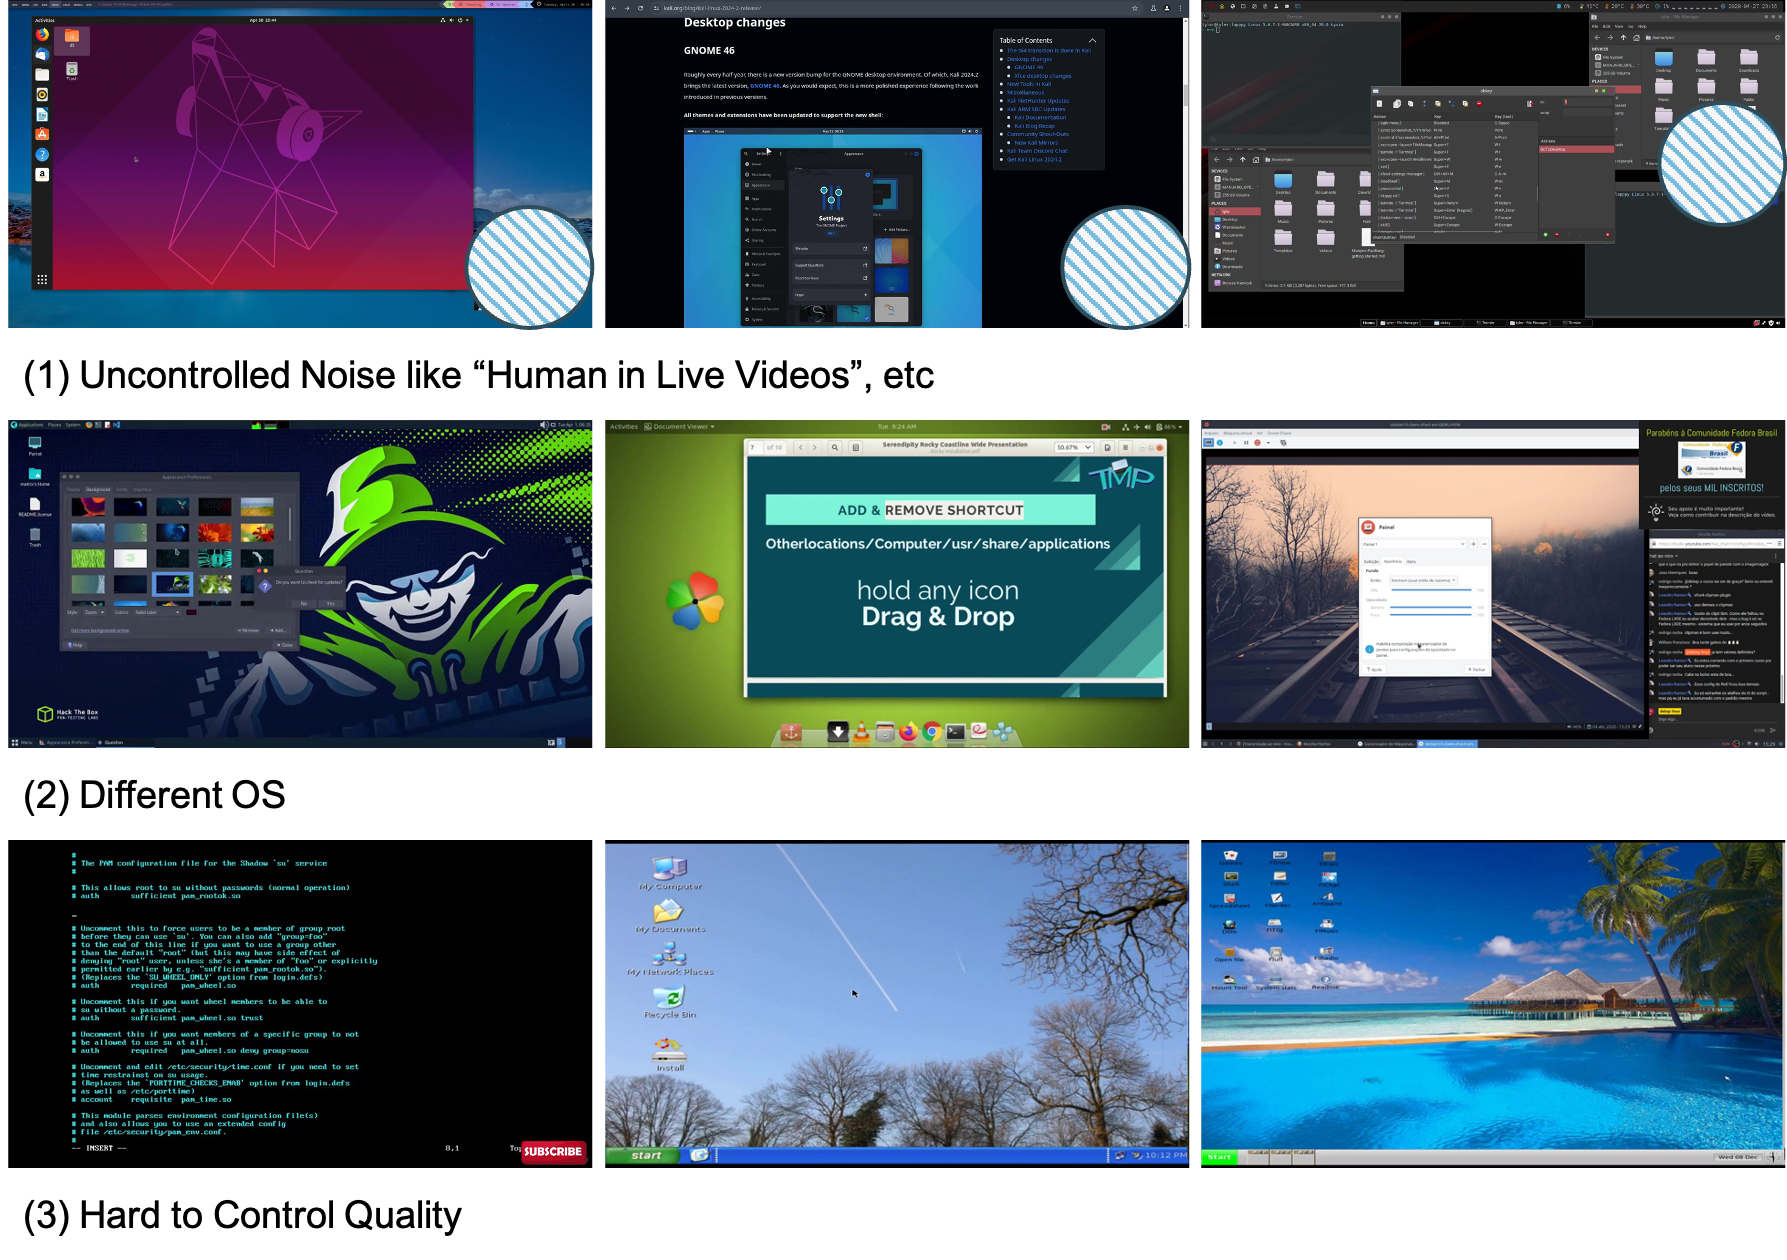
\includegraphics[width=\linewidth]{assets/web_data_issue.png}
  \vspace{-0.4em}
  \caption{\textbf{Common issues in web-scale screen video crawling.}
  Web videos mix uncontrolled content, heterogeneous OS/UI configurations, and inconsistent capture quality.
  This makes terminal localization, OCR, and time alignment unreliable without heavy filtering and sanitization.}
  \vspace{-10pt}
  \label{fig:web-video-issues}
\end{figure}

\subsection{Web video extraction}
We initially tested crawling computer-use videos from the web.
We used OCR and layout detectors to locate terminal regions, estimate text content and timestamps, and extract related clips.
We did not adopt this route for two main reasons:
\begin{tcolorbox}[
  colback=metablue!8,
  colframe=metablue!40,
  boxrule=0pt,
  borderline west={1pt}{0pt}{gray!60},
  left=6pt,right=4pt,top=3pt,bottom=3pt]
\small
\begin{itemize}
  \setlength{\itemsep}{2pt}
  \setlength{\topsep}{2pt}
  \item \textbf{Data governance constraints:} privacy and copyright risks are difficult to manage at web scale.
  \item \textbf{Data quality burden:} heavy filtering and sanitization are required before the data can support reliable OCR and temporal alignment.
\end{itemize}
\end{tcolorbox}
Screen recordings can contain personal identifiers (usernames, emails, file paths, chat content) and may come with licensing constraints that are difficult to verify at scale.
Cleaning the resulting data is substantially more complex than it appears (Figure~\ref{fig:web-video-issues}).
Typical failure modes include (i) uncontrolled content such as faces/hands, picture-in-picture overlays, and unrelated desktop activity;
(ii) domain shift across operating systems, themes, fonts, resolutions, and window managers; and
(iii) quality factors such as compression artifacts, variable frame rates, zoom/crop edits, and inconsistent capture pipelines.
These factors degrade OCR and temporal alignment.



Despite these challenges, web videos remain a potential long-term scaling axis for interface experience.
In this work, however, the cost--quality trade-off was unfavorable.
Our setting benefits disproportionately from clean, temporally aligned text and interaction signals.
Building a high-precision web filter also requires substantial upfront investment.
This includes rights-cleared sourcing or licensing, privacy review and redaction, and large-scale multimodal filtering/OCR pipelines that often rely on paid APIs.
Given these constraints and our emphasis on high-quality supervision, we prioritized curated, rights-cleared interface trajectories.
Future efforts that invest in rights-respecting acquisition and stronger automated filtering could unlock web-scale data as a complementary scaling axis.

\subsection{Online environment interaction}
We prototyped an agentic interaction pipeline that separates a control plane from an execution environment plane (Figure~\ref{fig:online-interaction-pipeline}).
In the environment plane, a sandboxed container runs a live shell together with LLM agents (planner/controller) and a recorder exposed via a narrow port-based interface.
The agents issue commands and control actions.
The recorder captures synchronized terminal renders, structured terminal state when available (e.g., buffer/text), and action traces.
Structured terminal state is logged for diagnostics/alignment and is not fed to video models as privileged state input.
Trajectories are streamed to the control plane for storage and video-model updates.

\begin{figure}[h]
  \centering
  \includesvg[inkscapelatex=false,width=\linewidth]{agentic_online_training}
  \vspace{-1.4em}
  \caption{\textbf{Agentic online interaction pipeline (early exploration).}
  A control plane ingests trajectories for storage and video-model updates (online where feasible, with offline replay support).
  A sandboxed environment plane executes an agent in an isolated container and records synchronized state/action traces.}
  \vspace{-10pt}
  \label{fig:online-interaction-pipeline}
\end{figure}


Concretely, the environment plane exposes a minimal ``step/reset'' interface over a port.
It returns multimodal observations that can be logged deterministically (rendered screenshots plus structured state when available).
The agent emits structured actions (typed command text, key/mouse events when applicable, and timing).
This separation makes rollouts auditable and lets the control plane scale rollout collection and model updates with decoupled throughput.

We explored this setup because closed-loop interaction can induce a natural curriculum by continually sampling the boundary of current video-model behavior.
It can also surface rare and safety-critical failure modes that do not appear in offline logs.
It supports targeted data collection (e.g., focusing on specific tools, error recovery, or long-horizon tasks).
In principle, it also offers a direct path to scaling \emph{experience} rather than only scaling static demonstrations.

Early trials showed promise, but the dominant bottlenecks in the end-to-end system were systems-level: cross-cluster communication latency between rollout workers and training nodes, and high debugging complexity in asynchronous distributed execution.
Safety controls (e.g., isolation of untrusted code execution, monitoring and abuse prevention, and deterministic resets and environment control) remained necessary constraints, but they were not the primary bottleneck.
The setup also requires robust recording and serialization across heterogeneous environments.
Under time and cost constraints, we therefore prioritized controlled video data for the main experiments. 
Despite not being used in the final pipeline, we consider this design a useful systems template for future work.
It supports scalable multi-environment rollout collection and consistent provenance and storage of trajectories.
It can support multiple downstream learning algorithms (e.g., behavior cloning or preference-based learning).
Execution remains sandboxed and auditable.


\newpage
\section{Datasets: Collection and Evaluation Protocols}
\label{appendix:pipeline}
\noindent This appendix summarizes collection, preprocessing, and evaluation details for the datasets used in the paper.
For concrete examples of raw trajectory formats (asciinema \texttt{.cast} and \texttt{vhs} scripts), see Appendix~\ref{appendix:cligen-samples}. 
% 
Data collection uses a three-stage pipeline to maintain synchronized timing, privacy controls, and consistent, well-documented artifacts across CLIGen and GUIWorld.

\noindent\textbf{Sourcing.}
We construct our datasets from three complementary sources---public terminal recordings, scripted terminal replays, and a controlled desktop-capture rig.
Across all sources, we emphasize rights-respecting acquisition, privacy filtering, and temporally aligned interface signals (frames, actions, and text when available):
\begin{tcolorbox}[
  colback=metablue!8,
  colframe=metablue!40,
  boxrule=0pt,
  borderline west={1pt}{0pt}{gray!60},
  left=6pt,right=4pt,top=3pt,bottom=3pt]
\small
\begin{itemize}
  \setlength{\itemsep}{2pt}
  \setlength{\topsep}{2pt}
  \item \cligenGeneralLogo{}\,\textbf{CLIGen (General)}: public \texttt{asciinema} \texttt{.cast} archives; traces are replayed with official tools to preserve recorded terminal appearance (color schemes, cursor visibility, window geometry).
  \item \cligenCleanLogo{}\,\textbf{CLIGen (Clean)}: deterministic \texttt{vhs} scripts (e.g., package installs, REPLs, log filters) executed in isolated environments.
  \item \guiworldLogo{}\,\textbf{GUIWorld}: footage captured with the rig in \Cref{section:impl-guiworld}, pairing RGB video with low-latency pointer/key logs and optional accessibility cues (logged for analysis; not used as model inputs).
\end{itemize}
\end{tcolorbox}

\noindent\textbf{Alignment and sanitization.} 
All modalities share a common clock.
We align pointer/key events to the nearest frame, apply drift correction when needed, and drop clips with residual misalignment.
Privacy filters remove terminal sessions with sensitive strings and redact GUI regions likely to contain private content.
Frozen or repeated-frame recordings (capture artifacts) are discarded.

\noindent\textbf{Episode packaging.}
Runs are windowed into fixed-length, overlapping episodes (window sizes and strides are specified in the released configs).
Each shard stores RGB frames, terminal buffers or GUI metadata, serialized actions, the source tool (\texttt{asciinema}/\texttt{vhs}/GUI capture), and environment metadata.
Structured fields (buffers/metadata) are used for alignment and evaluation, but are not provided to the video models as state inputs.
Downstream dataloaders reconstruct batches directly.
Released configs specify preprocessing and windowing so external users can rebuild the corpus.

\subsection{Caption fields and metadata (CLIGen General)}
For CLIGen (General), each replayed \texttt{.cast} fragment (example shown in \Cref{appendix:cast-format}) is paired with three aligned descriptions and a compact metadata record.
Table~\ref{tab:cast-captions} summarizes the fields for clip \texttt{7****\_0001}.

\begin{smallschemetable}{Caption tiers and metadata for CLIGen (General) clip \texttt{7****\_0001}.}{tab:cast-captions}
  \rowcolors{2}{metablue!8}{white}
  \begin{tabularx}{\linewidth}{@{}l X@{}}
    \toprule
    \rowcolor{metablue!16}\textbf{Field} & \textbf{Content (abridged)} \\
    \texttt{caption} &
      The user (username field shown verbatim as \texttt{annonomous} [sic]) logged into their account on the host \texttt{NeuralComputer}, and after some initial terminal setup and cursor movements,
      they started typing the command \texttt{nvim} to likely open the Neovim text editor, but the session recording ends abruptly without showing the actual command execution or any further interaction. \\
    \texttt{caption\_detailed} &
      At the \texttt{annonomous@NeuralComputer:~\$} prompt, the user types \texttt{nvim}, but before the command executes, the screen rapidly displays a colorful,
      pixelated animation with various RGB colors, including shades of blue, green, and purple, filling the 80x24 terminal window.
      The animation is briefly interrupted by a cursor blink, then the prompt returns, awaiting further input. \\
    \texttt{caption\_semantic} &
      The terminal displays a rapid sequence of colored text and pixel art animations, with syntax-highlighted code and prompts appearing in a mix of blue, green,
      and white hues, as the user types commands and the system responds with scrolling output, error messages, and success indicators. \\
    \midrule
    \texttt{data\_info.version} & \texttt{2} (\texttt{asciinema} v2 header) \\
    \texttt{data\_info.size} & \texttt{width=80}, \texttt{height=24}; original/target/scaled sizes all match, padding \texttt{[0,0]}. \\
    \texttt{data\_info.env} & \texttt{SHELL=/bin/bash}, \texttt{TERM=xterm-256color}. \\
    \texttt{meta.videogen} &
      Automatically derived stats: visual complexity \texttt{2897.7}, interaction density \texttt{1.0}, color usage \texttt{518}, screen clears \texttt{6},
      event rate \texttt{7.8} events/s, typing rhythm (avg interval \texttt{0.13}s, variance \texttt{0.34}), and \texttt{38} visual-change events. \\
    \texttt{metadata} &
      Source recording on Asciinema: id \texttt{7****}, title \texttt{``aneo.nvim demo''}, author \texttt{annonomous} [sic], creation time \texttt{2025-05-13T23:37:53Z}, URLs for the page and raw \texttt{.cast}. \\
    \bottomrule
  \end{tabularx}
\end{smallschemetable}

These fields make each CLIGen (General) clip self-contained.
The three caption tiers provide prompts at different levels of detail.
\texttt{data\_info} and \texttt{metadata} preserve the structure needed to rebuild terminal geometry, environment, and source from the raw \texttt{.cast}. 
% A heuristic category count indicates that the dataset covers diverse terminal usage.
% It includes general terminal operations (610,331 clips), file operations (81,783), programming activities (66,430), system administration (42,668), and text editing (22,777).
% This distribution reflects typical command-line workflows across different user tasks.

\subsection{OCR evaluation protocol (CLIGen Clean)}
For CLIGen (Clean), OCR-based metrics evaluate how closely generated terminal videos match reference renderings derived from the ground-truth buffers in text space rather than pixels.
Each sample consists of a generated video and its paired reference video (matched by clip ID).
We keep only IDs where both videos are present. 
% 
From each paired video we use at most $K{=}5$ frames.
Let $T_\text{gen}$ and $T_\text{gt}$ be the frame counts of the generated and reference videos.
We set $T=\min(T_\text{gen},T_\text{gt})$.
If $T \le K$, we use all indices in $[0, T{-}1]$; otherwise, we select $K$ evenly spaced indices by deterministic rounding, then deduplicate and sort them so evaluation frames are spread across the trajectory.
For every selected index we read the corresponding frame from both videos.

Each frame is converted to RGB and passed to Tesseract OCR.
The resulting string is split into lines, leading and trailing whitespace is stripped, and internal whitespace is normalized by collapsing runs of spaces.
Empty lines are dropped.
We keep case and punctuation intact so that commands, paths, and symbols remain visible.
This gives an ordered list of normalized lines for the ground-truth frame ($g_1,\dots,g_{N_g}$) and the generated frame ($p_1,\dots,p_{N_p}$).

We summarize the OCR text-space metrics used per sampled frame as follows:
\begin{tcolorbox}[
  colback=metablue!8,
  colframe=metablue!40,
  boxrule=0pt,
  borderline west={1pt}{0pt}{gray!60},
  left=6pt,right=4pt,top=3pt,bottom=3pt]
\small
\textbf{Character accuracy.} This metric pools all lines into a single multi-line string for each side and measures normalized edit distance.
Let $s$ and $t$ be the concatenated ground-truth and generated texts and $d(s,t)$ their Levenshtein distance (insert/delete/replace cost $1$).
If both $s$ and $t$ are empty we set $\text{char\_acc}=1$; if only $s$ is empty we set $\text{char\_acc}=0$.
Otherwise,
\[
  \text{char\_acc} = \max\Bigl(0,\ 1 - \frac{d(s,t)}{\max(|s|,1)}\Bigr),
\]
Extra or missing characters are normalized by the reference length through the denominator $\max(|s|,1)$.
Frame-level scores are averaged over the selected frame pairs (up to $K{=}5$) to yield a per-video character accuracy, and group-level scores report the mean over videos.

\textbf{Exact-line accuracy.} This metric treats lines as position-sensitive units and reports a recall over ground-truth lines.
For a given frame, we compare line $g_i$ to $p_i$ at the same index.
A line is counted as correct only if $i\le N_p$ and $p_i=g_i$; lines that appear in the wrong position do not count.
If both lists are empty we set $\text{exact\_line\_acc}=1$; if the ground-truth list is empty but the generated list is not, we set $\text{exact\_line\_acc}=0$.
Otherwise,
\[
  \text{exact\_line\_acc} = \frac{1}{N_g}\sum_{i=1}^{N_g} \mathbf{1}[i \le N_p \land p_i = g_i].
\]
As with character accuracy, frame scores are averaged over the $K$ sampled frames to obtain a per-video score and then averaged over videos for the reported aggregate.
\end{tcolorbox} 
% Unless otherwise noted, OCR results in the main text use 1,000 randomly sampled video pairs (five frame pairs per video).
Together, these two metrics stress both fine-grained text fidelity and line-ordered terminal state reconstruction.

\subsection{Evaluation metrics and protocol (GUIWorld)}
\label{appendix:gui-metrics}
We report both global video metrics and action-driven metrics that focus on post-interaction frames. 
We compute these metrics using our GUIWorld evaluation suite.
We summarize the GUIWorld protocol at a glance as follows:
\begin{tcolorbox}[
  colback=metablue!8,
  colframe=metablue!40,
  boxrule=0pt,
  borderline west={1pt}{0pt}{gray!60},
  left=6pt,right=4pt,top=3pt,bottom=3pt]
\small
\begin{itemize}
  \setlength{\itemsep}{2pt}
  \setlength{\topsep}{2pt}
  \item \textbf{Global metrics} (\FVD$_\text{all}$, \SSIM$_\text{all}$, \LPIPS$_\text{all}$): computed over paired generated/ground-truth videos after standardized decoding, subsampling, and resizing.
  \item \textbf{Action-driven metrics} (\SSIM$_{+15}$, \LPIPS$_{+15}$, \FVD$_{+15}$): computed on post-action windows to measure interface fidelity after interaction events.
\end{itemize}
\end{tcolorbox}

\noindent\textbf{Global \FVD$_\text{all}$/\SSIM$_\text{all}$/\LPIPS$_\text{all}$}
We decode paired generated/ground-truth videos into RGB frames with temporal subsampling and resizing (\texttt{fps}=3, \texttt{size}=256, and \texttt{max\_seconds}=5 by default).
\SSIM$_\text{all}$~is computed using \texttt{torchmetrics} on frame tensors normalized to $[0,1]$ and averaged over frames.
\LPIPS$_\text{all}$~uses the AlexNet backbone on frames normalized to $[-1,1]$ and is averaged over frames.
\FVD$_\text{all}$~is computed in an \texttt{r3d18} embedding space (\texttt{prelogits} by default).
We extract features from fixed-length clips (16 frames at 112$\times$112 after uniform subsampling/padding).
We compute the Fr\'echet distance between the generated and reference feature distributions.

\noindent\textbf{Action-driven metrics (\SSIM$_{+15}$, \LPIPS$_{+15}$, \FVD$_{+15}$)}
For each paired rollout, we load recorded action timestamps (from JSON/CSV logs), map each timestamp $\tau$ to a frame index $f=\mathrm{round}(\tau \cdot \mathrm{fps})$, and clamp to the valid frame range.
We skip the action frame itself (\texttt{action\_start\_offset}=1) and evaluate the next $k{=}15$ frames after each action.
Concretely, for each action frame index $f$, we form the post-action set $\{f+1,\dots,f+k\}$ and clip it to valid frame indices.
We then take the deduplicated union over actions in the clip and keep frame indices in chronological order.
Clips with zero logged actions, or with empty valid post-action windows after clipping, are excluded from $+15$ metrics.
For \SSIM$_{+15}$~/\LPIPS$_{+15}$, we compute per-clip means over selected frame pairs and then average across clips.
For action-driven \FVD$_{+15}$, we build an \emph{after-action clip} per video by concatenating the same selected post-action frames, then uniformly subsample/pad to 16 frames and compute the Fr\'echet distance in the same \texttt{r3d18} feature space.


\newpage
\section{CLIGen: CLI Trajectory Formats}
\label{appendix:cligen-samples}
\noindent This appendix provides concrete format examples for the two CLI sources referenced throughout the data pipeline (Appendix~\ref{appendix:pipeline}).
We show asciinema \texttt{.cast} trajectories for CLIGen (General) and \texttt{vhs} scripts for CLIGen (Clean).
\subsection{Asciinema (\texttt{.cast}) example}
\label{appendix:cast-format}
The header line stores the recording config (version, terminal size, timestamp, env).
In this excerpt, output rows follow \texttt{[time, "o", "payload"]}, where \texttt{"o"} indicates screen output.
The payload contains the terminal text with color codes at that timestamp.
\begin{verbatim}
{"version": 2, "width": 80, "height": 24,
 "timestamp": 1747177906,
 "env": {"SHELL": "/bin/bash", "TERM": "xterm-256color"}}
[0.082492, "o", "\u001b[H\u001b[2J\u001b[3J"]
[0.950038, "o", "\u001b[38;2;16;131;236m\u001b[39m\r\n..."]
[0.950733, "o", "\u001b[38;2;6;156;220m ... \u001b[38;2;1;195;187m█"]
\end{verbatim}

\subsection{VHS script example}
\label{appendix:vhs-format}
\begin{verbatim}
# ---- VHS documentation start (DO NOT CHANGE) ----
# Require:
#   Require <string>
# Sleep:
#   Sleep <time>
# Type:
#   Type[@<time>] "<characters>"
# Keys:
#   Escape[@<time>] [number]
#   Backspace[@<time>] [number]
#   Delete[@<time>] [number]
#   Insert[@<time>] [number]
#   Down[@<time>] [number]
#   Enter[@<time>] [number]
#   Space[@<time>] [number]
#   Tab[@<time>] [number]
#   Left[@<time>] [number]
#   Right[@<time>] [number]
#   Up[@<time>] [number]
#   PageUp[@<time>] [number]
#   PageDown[@<time>] [number]
#   ctrl+<key>
# Display:
#   Hide
#   Show
# ---- VHS documentation end (DO NOT CHANGE) ----

# ID: vhs_example
# INSTRUCTION: Runs `uname -s` repeatedly as a basic shell exercise, then hides the prompt.
# LEVEL: 1
# EVENTS: 23
# VISUAL_COMPLEXITY: 45

# ---- Theme setting start (DO NOT CHANGE) ----
Output vhs_example.mp4

Set Shell "bash"

Set Theme {
  "name": "Catppuccin Mocha (Pure White, Warm Pink Cursor)",
  "background": "#1e1e2e",
  "foreground": "#ffffff",
  "black": "#45475a",
  "red": "#f38ba8",
  "green": "#a6e3a1",
  "yellow": "#f9e2af",
  "blue": "#89b4fa",
  "purple": "#cba6f7",
  "cyan": "#94e2d5",
  "white": "#ffffff",
  "brightBlack": "#585b70",
  "brightRed": "#f38ba8",
  "brightGreen": "#a6e3a1",
  "brightYellow": "#f9e2af",
  "brightBlue": "#89b4fa",
  "brightPurple": "#cba6f7",
  "brightCyan": "#89dceb",
  "brightWhite": "#ffffff",
  "cursor": "#f5c2e7",
  "cursorAccent": "#1e1e2e",
  "selectionBackground": "#585b70"
}

Set FontSize 40
Set Width 1600
Set Height 900
Set TypingSpeed 300ms
Set PlaybackSpeed 1
Set Margin 28
Set MarginFill "#0091FF"
Set BorderRadius 25
Set Padding 18
Set LineHeight 1.2
Set LetterSpacing 0.8
# ---- Theme setting end (DO NOT CHANGE) ----

Sleep 800ms
Sleep 180ms
Type "uname -s"
Sleep 120ms
Enter
Sleep 400ms
Type "uname -s"
Sleep 120ms
Enter
Sleep 400ms
Type "uname -s"
Sleep 120ms
Enter
Sleep 400ms
Type "uname -s"
Sleep 120ms
Enter
Sleep 400ms
Type "uname -s"
Sleep 120ms
Enter
Sleep 400ms
Sleep 400ms
Sleep 600ms
Hide
\end{verbatim}


\newpage
\section{GUIWorld: Action Representation, Temporal Alignment, and Conditioning}
\label{appendix:gui-actions}
\noindent This appendix provides additional technical details on GUIWorld action representation, temporal alignment, and conditioning used in Section~\ref{section:impl-guiworld}.
Additional visualization pages are collected in Appendix~\ref{appendix:vis}; evaluation metrics and protocols are summarized in Appendix~\ref{appendix:gui-metrics}.

\subsection{Action schema}
\ncguiworld{} represents actions as a structured stream, enabling the NC to condition on both cursor movements and key presses.

At each timestep, we log absolute cursor coordinates, button up/down transitions, scroll deltas, and keyboard events.
Keyboard inputs are split into two types: typed characters (e.g., \texttt{ls -l}) and shortcut-style chords (e.g., \texttt{ctrl+v}).
We also track state flags such as whether a drag is currently active.
This lets us represent extended interactions like click-drag or press-hold as short labeled segments rather than isolated spikes.
The meta-action encoder described in Section~\ref{section:impl-guiworld} compresses this stream into a small typed schema.
In all reported v2 experiments, we use $S{=}2$ action slots per frame; empty slots are padded with type~0.
Each action has a type (e.g., \texttt{mouse click} or \texttt{keyboard type}) plus parameters.
Table~\ref{tab:meta-action-schema} summarizes the types and fields.
Type~0 corresponds to the absence of an action.
Type~1 encodes mouse clicks and drags via button identity, click count, and a drag flag.
Type~2 captures scrolls with a direction and scalar amount.
Type~3 packages free-form keyboard text (such as \texttt{ls -l}) embedded by the shared text encoder.
Type~4 records shortcuts such as \texttt{ctrl+v} via a small shortcut vocabulary.
This representation resembles a tool API while remaining recoverable from raw logs.

\begin{table}[h]
  \centering
  \small
  \setlength{\tabcolsep}{6pt}
  \renewcommand{\arraystretch}{1.05}
  \caption{Meta-action schema for GUIWorld (per action slot).}
  \label{tab:meta-action-schema}
  \rowcolors{2}{metablue!8}{white}
  \begin{tabularx}{\linewidth}{@{}c l >{\raggedright\arraybackslash}X@{}}
    \toprule
    \rowcolor{metablue!16}\textbf{Type id} & \textbf{Action} & \textbf{Parameter fields} \\
    0 & None & -- \\
    1 & Mouse Click/Drag & \texttt{button}, \texttt{click\_count}, \texttt{drag\_flag} \\
    2 & Mouse Scroll & \texttt{direction}, \texttt{amount} \\
    3 & Keyboard Type & \texttt{text} (e.g., \texttt{ls -l}) $\rightarrow$ shared text encoder \\
    4 & Shortcut & \texttt{shortcut\_id} (e.g., \texttt{ctrl+v}) \\
    \bottomrule
  \end{tabularx}
\end{table}

\subsection{Conditioning: encoders and injection}
The main text considers two encoders for this stream.
A \emph{raw-action encoder (v1)} keeps fine-grained mouse and key events in a multi-hot representation that closely mirrors real cursor and typing behavior.
A complementary \emph{meta-action encoder (v2)} compresses events into a small typed schema (Table~\ref{tab:meta-action-schema}) and embeds any free-form text with a shared text encoder.
Both encoders produce per-frame action features that undergo temporal windowing and alignment (described below).
These embeddings support four injection modes, summarized below:
\begin{tcolorbox}[
  colback=metablue!8,
  colframe=metablue!40,
  boxrule=0pt,
  borderline west={1pt}{0pt}{gray!60},
  left=6pt,right=4pt,top=3pt,bottom=3pt]
\small
\begin{itemize}
  \setlength{\itemsep}{2pt}
  \setlength{\topsep}{2pt}
  \item \texttt{external}: fuse actions at the VAE input.
  \item \texttt{contextual}: mix actions and frames as tokens in one sequence.
  \item \texttt{internal}: inject actions inside transformer blocks.
  \item \texttt{residual}: add lightweight action deltas to hidden states.
\end{itemize}
\end{tcolorbox}

\noindent\textbf{Injection-mode definitions (schematic)}
\label{appendix:gui-injection-equations}
Below we give compact schematic definitions for the three formula-based modes (\texttt{external}, \texttt{residual}, \texttt{internal}); \texttt{contextual} is specified by the structured attention mask in Figure~\ref{fig:contextual-mask}.
%
\textbf{External.} Given VAE latents $z_{1:T}$ and temporally aligned action features $u_{1:T}$, an external action module produces a residual update $\Delta z_{1:T}(u_{1:T})$ and forms modified latents
\[
  z'_{1:T} = z_{1:T} + \Delta z_{1:T}(u_{1:T}).
\]
The diffusion backbone then operates on $z'_{1:T}$ (actions do not appear as explicit tokens inside the transformer).
%
\textbf{Residual.} At selected transformer layers $l$, an auxiliary action module takes block hidden states $h^{(l)}$ together with local action/mouse features and outputs a residual update $\Delta h^{(l)}(a,\text{mouse})$.
The updated hidden states are
\[
  \tilde{h}^{(l)} = h^{(l)} + \Delta h^{(l)}(a,\text{mouse}),
\]
which are passed to the next block.

\textbf{Internal.} At selected blocks, action conditioning is inserted as an additional cross-attention sub-layer inside the standard attention stack.
With self-attention $\mathrm{SA}$, text/reference cross-attention $\mathrm{CA}_{\text{text}}$, and action cross-attention $\mathrm{CA}_{\text{action}}$, a schematic update is
\[
  h' = \mathrm{FFN}\Big(
    h + \mathrm{CA}_{\text{text}}\big(\mathrm{SA}(h), c\big)
      + \mathrm{CA}_{\text{action}}(h, a)
  \Big).
\]

\subsection{Temporal alignment and attention}
\noindent\textbf{Temporal alignment and windows.}
The GUI backbone processes a compressed latent video at stride $c$ (every $c$ pixel frames correspond to one latent frame).
For a pixel sequence of length $F$ and latent sequence of length $T$, we approximately have $F \approx (T-1)c + 1$ under uniform sampling.
Exact indexing follows the dataloader timestamp mapping and boundary handling.
Anchor frame $a_t = t \cdot c$ marks the pixel frame corresponding to latent step $t$.

Mouse and keyboard logs start as per-frame features $r_f \in \mathbb{R}^D$ at the pixel rate.
A windowed encoder aggregates them around each anchor over $p = c \cdot w$ frames.
Here $w$ controls the window width, and a lag $\ell$ accounts for GUI response delay (actions precede their visual effects).
We use zero-padding outside the valid range, i.e., $\tilde{r}_f=r_f$ for $0\le f<F$ and $\tilde{r}_f=0$ otherwise, and form a lag-shifted window that ends at $a_t-\ell$:
\[
  W_{t,k} = \tilde{r}_{\,a_t - (p-1+\ell) + k}, \quad k\in\{0,\dots,p-1\}, \quad
  a^{\text{act}}_t = \frac{1}{p} \sum_{k=0}^{p-1} W_{t,k}.
\]
This shared action encoder yields one latent-aligned action embedding $a^{\text{act}}_t$ per step.
It summarizes a short, lagged history of cursor motion and key events and is reused across all injection modes.

\noindent\textbf{Contextual attention mask.}
In the \texttt{contextual} mode, video and action tokens are concatenated into a single sequence and processed under a structured lag-aware local attention mask.
Appendix Figure~\ref{fig:contextual-mask} can be read as a query--key matrix: rows are queries and columns are keys.

The upper-left block (\emph{V2V}) restricts each frame $V_i$ to attend only to neighboring frames within a window of $\pm w$ steps, so very distant frames cannot interfere.
The upper-right block (\emph{V2A}) lets frame $V_i$ see only recent actions in a lag-bounded recent-action range.
In implementation, this window is $j \in [\max(0, i-\ell), \min(i, A-1)]$, where $\ell$ is the action lag and $A$ is the action-token length.
This way, frame conditioning stays focused on recent operations and excludes future actions.
In the lower-left block (\emph{A2V}), an action $A_i$ can attend to frames $V_t$ that occur after it has had time to take effect ($t \ge i+\ell$, with boundary clipping), but not to earlier frames.
This path is representation-only and does not expose future frame information to frame prediction.
The lower-right block (\emph{A2A}) is strict diagonal: each action token attends to itself.

In practice $(w,\ell)$ act as fixed hyperparameters that trade off temporal coverage and cost.
Together, these choices implement a structured lag-aware temporal prior: actions do not explain past frames, and each frame conditions on recent operations that could plausibly have shaped its pixels.

\noindent\textbf{Design insights.} Two insights from the GUI experiments motivate this schema.
First, raw action streams are bursty and high-dimensional.
Cursor and key events arrive in short spikes, and simple smoothing or full-history attention can cause false interpolated motion and underestimated typing speed.
Using short, lagged windows and local attention bands makes credit assignment more intuitive: each frame connects to the few operations that could have produced it.
Second, in our experiments, with the visual backbone fixed, control fidelity improved more from conditioning design than from encoder choice.
Clean, well-paced supervision and mid- or deep-level action injection improve cursor accuracy and hover timing, while different encodings of the same stream perform similarly.
This action schema and mask implement these principles: keep pixels and actions aligned in time, prioritize recent operations over distant ones, and use attention structure rather than~capacity~alone.

\subsection{Cursor rendering and supervision}
\noindent\textbf{Cursor rendering and reference construction.}
\label{appendix:cursor-rendering} 
%
The cursor pipeline applies the same design principles on the visual side.
Instead of relying on the global diffusion loss to recover a small, high-frequency visual target, we render the cursor explicitly.
We treat it as a first-class conditioning signal.

\noindent\textbf{From logs to normalized trajectories.}
\label{appendix:mouse-traj-normalization}
Desktop logs provide per-frame cursor positions in screen coordinates $(x_\text{screen},y_\text{screen})$ at the native GUI resolution.
We align these with sampled video frames using the same letterbox mapping as the RGB stream.
Given source and target resolutions $(w_\text{src}, h_\text{src})$ and $(w_\text{dst}, h_\text{dst})$, we compute a uniform scale $s$ and padding offsets $(p_x,p_y)$.
Each coordinate is then mapped to normalized positions $(x_t,y_t)\in[0,1]^2$ as
\[
  x_t = \frac{s\,x_{\text{screen},t} + p_x}{w_\text{dst}-1},\qquad
  y_t = \frac{s\,y_{\text{screen},t} + p_y}{h_\text{dst}-1}.
\]
Stacking these over time yields the trajectory tensor \texttt{mouse\_trajectories} used across rendering and action encoding.


\begin{table}[h!]
  \centering
  \small
  \setlength{\tabcolsep}{4pt}
  \renewcommand{\arraystretch}{1.12}
  \caption{Raw-action versus meta-action encoders in GUIWorld.}
  \label{tab:action-encoder-comparison}
  \begin{tabularx}{\linewidth}{p{2.9cm} >{\raggedright\arraybackslash}X >{\raggedright\arraybackslash}X}
    \toprule
    \textbf{Aspect} &
    \textbf{Raw-action encoder (v1)} &
    \textbf{Meta-action encoder (v2)} \\
    \midrule
    \textbf{Action schema} &
    Per-frame multi-hot vector composed of
    13 mouse actions and 169 keyboard actions;
    no explicit type hierarchy. &
    Hierarchical schema with explicit action types and parameters:
    \texttt{action\_types} $\in \{0,1,2,3,4\}$ for
    \{None, Mouse Click/Drag, Mouse Scroll, Keyboard Type, Keyboard Shortcut\},
    plus typed parameter fields (e.g., button, scroll amount, shortcut ID, text). \\[2pt]
    %
    \textbf{Mouse representation} &
    Two signals per frame:
    (1) continuous cursor trajectory
    $\texttt{mouse\_trajectories}_{t} \in \mathbb{R}^2$;
    (2) discrete mouse events
    $\texttt{mouse\_action\_events}_{t} \in \{0,1\}^{13}$ (multi-hot). &
    Per-frame mouse trajectory
    $\texttt{mouse\_trajectories}_{t}$
    is encoded by a shared mouse-trajectory encoder and the temporal windowing module into
    dense mouse embeddings
    $\texttt{mouse\_latent}_{t} \in \mathbb{R}^{d_{\text{mouse}}}$,
    optionally fused with action embeddings. \\[2pt]
    %
    \textbf{Keyboard representation} &
    Per-frame keyboard state
    $\texttt{keyboard\_action\_events}_{t} \in \{0,1\}^{169}$,
    where each dimension corresponds to a key or shortcut;
    only multi-hot activation is available, no text semantics. &
    Two complementary forms:
    keyboard shortcuts as
    \texttt{keyboard\_shortcut} IDs embedded via an embedding table, and
    free-form text \texttt{keyboard\_text} (e.g.\ ``ls -l'')
    encoded by a shared text encoder (e.g., T5) and projected to the
    action embedding dimension. \\[2pt]
    %
    \textbf{Per-frame representation} &
    Mouse and keyboard events are concatenated:
    $\texttt{raw\_actions}_{t}
      = [\,\texttt{mouse\_events}_{t},\,
           \texttt{keyboard\_events}_{t}\,]
      \in \mathbb{R}^{182}$. &
    For each frame $t$ and slot $s$,
    type plus parameters are embedded into
    \texttt{slot\_embeds}$_{t,s} \in \mathbb{R}^{D}$.
    Valid slots are aggregated (mean or attention) into a single
    per-frame action embedding
    $\texttt{action\_embeds}_{t} \in \mathbb{R}^{D}$. \\[2pt]
    %
    \textbf{Multi-slot support} &
    No explicit notion of multiple action slots per frame;
    all mouse and keyboard signals are collapsed into one
    182-d multi-hot vector. &
    Explicit multi-slot design:
    \texttt{action\_types} and all parameter tensors have shape
    $(B, T, S)$ with $S=2$ slots per frame,
    enabling, e.g., concurrent ``mouse click + keyboard shortcut''
    in the same frame. \\[2pt]
    %
    \textbf{Latent-aligned representation} &
    Temporal alignment is implemented ad-hoc inside each
    v1 action module (e.g., sliding windows over the
    182-d per-frame vector),
    with custom logic per mode (external, internal, residual). &
    A unified temporal alignment module takes per-frame action embeddings
    $(B, F, D)$ and VAE compression ratio $c$,
    constructs lag-aware temporal windows of size
    $c \cdot w$,
    and outputs latent-aligned action features
    $\texttt{action\_latent} \in \mathbb{R}^{B \times T \times D}$,
    with analogous $\texttt{mouse\_latent}$ when mouse features are enabled. \\[2pt]
    %
    \textbf{Lag modeling} &
    GUI latency / response lag is implicitly encoded
    by where and how the sliding window is applied
    inside each v1 action module; there is no shared
    lag configuration across modes. &
    Lag is an explicit hyperparameter
    \texttt{action\_lag} in the temporal alignment and in
    the contextual attention mask:
    it shifts temporal windows and defines which frames
    an action can attend to, giving a consistent lag interpretation across modes. \\[2pt]
    %
    \textbf{Downstream usage} &
    Raw 182-d vectors (plus trajectories) are fed directly into the v1 action modules (external, internal, residual) without a shared temporal encoder. &
    The v2 encoder outputs provide a shared conditioning stream for all v2 modes and also supply features for the temporal contrastive loss. \\[2pt]
    %
    \textbf{Contrastive supervision} &
    No dedicated temporal contrastive loss between frames
    and actions; supervision comes only from the generative objective. &
    Action and mouse latents are coupled to frame features via
    an InfoNCE-style temporal contrastive loss, encouraging time-aligned action embeddings. \\
    \bottomrule
  \end{tabularx}
\end{table}


\subsection{Training signals and encoder design}

\noindent\textbf{From trajectories to cursor layers.}
Starting from normalized $(x_t,y_t)$ coordinates, a cursor-layer module renders a fixed SVG arrow template into RGB and alpha channels.
The template is reused across frames.
For each timestep $t$, it is positioned so the hotspot (arrow tip) aligns with $(x_t,y_t)$, clipped to screen bounds, and alpha-blended over a neutral background.
This produces two tensors at video frame rate: a cursor-only foreground image $f_t \in [-1,1]^{3\times H \times W}$ and a soft mask $m_t \in [0,1]^{1\times H \times W}$ isolating the arrow pixels.
Invalid or missing coordinates zero the mask and leave the foreground unchanged, so frames without visible cursors do not add spurious supervision.

\noindent\textbf{Reference images and masks.}
These cursor layers become reference conditions for the image-to-video (I2V) model.
For each clip we form reference images $\mathrm{ref\_img}_{0:T-1}$ and masks $\mathrm{ref\_mask}_{0:T-1}$:
\begin{itemize}
  \item At $t{=}0$, $\mathrm{ref\_img}_0$ is the full desktop frame and $\mathrm{ref\_mask}_0$ is all ones, anchoring the static layout and theme;
  \item For $t{>}0$, $\mathrm{ref\_img}_t$ is the cursor foreground $f_t$ and $\mathrm{ref\_mask}_t$ is the cursor mask $m_t$, so only the arrow region is supervised while the background remains free.
\end{itemize}
The model encodes these references with the same VAE as target frames and concatenates their latents and masks into the diffusion input.
It enforces masked, reference-consistent reconstruction inside the cursor region while relying on learned dynamics elsewhere.
This makes cursor supervision a pixel-level constraint rather than a side effect of the global loss.

\noindent\textbf{Fourier mouse encoding.}
The same $(x_t,y_t)$ trajectories serve as a continuous control signal.
We apply a Fourier position module: clamp coordinates to $[0,1]^2$, map them to $[-1,1]^2$, and compute random Fourier features via a fixed Gaussian projection followed by sine/cosine.
A small MLP maps these features to per-frame mouse embeddings.
The GUIWorld action encoder then aggregates them with lag-aware, stride-aligned windows to produce latent-aligned mouse features.
These features condition the \texttt{external}/\texttt{contextual}/\texttt{residual}/\texttt{internal} modes and participate in the temporal contrastive loss.

\noindent\textbf{Cursor-aware losses.}
Section~\ref{section:impl-guiworld} introduces cursor-aware losses that use this construction.
A basic variant penalizes position error only in $(x,y)$.
Richer variants add Fourier features of the trajectory and, most importantly, an $\ell_2$ loss on the reconstructed cursor patch under $\mathrm{ref\_mask}_t$.
Table~\ref{tab:cursor-loss} shows that position-only objectives yield low cursor hit rate and visibly jittery arrows even when videos look plausible.
Adding the explicit cursor reference stream together with the masked patch loss substantially improves control, reaching 98.7\% cursor accuracy.
This confirms that explicit cursor rendering plus localized supervision effectively separates ``where the arrow is'' from ``what the rest of the frame should look like''.

\noindent\textbf{Temporal contrastive alignment.}
To strengthen learning signals for the action pathway, we add a lightweight temporal contrastive loss that operates on the same latent timeline as the diffusion model.
For each sequence we take per-step frame features $F_{t} \in \mathbb{R}^{d_f}$ pooled from the latent video.
We also take per-step action features $A_{t} \in \mathbb{R}^{d_a}$ and (optionally) mouse features $M_{t} \in \mathbb{R}^{d_m}$ produced by the action encoder.
Linear projections map these into a common space and the resulting vectors are $\ell_2$-normalized.
An InfoNCE-style objective brings matching pairs $(F_t,A_t)$ (and, when present, $(F_t,M_t)$) from the same timestep together.
In implementation, matching is lag-aware: frame $t$ is aligned with action/mouse features at $t-\ell$, where $\ell$ is the configured \texttt{action\_lag}.
Similarities are scaled by a temperature $\tau$.
It pushes matched pairs away from other timesteps of the \emph{same} sequence.
We use frame and action masks to ignore positions without actions.
A symmetric variant averages frame-to-action and action-to-frame directions.

When enabled, a small future-prediction head adds a second term.
Action features at time $t$ are mapped to a prediction of the frame feature at a slightly later step $t+\ell$.
A mean-squared error encourages consistency between the prediction and the projected future frame.
Together, these terms give the action encoder direct gradients tied to specific frames rather than relying solely on the pixel diffusion loss.
The contrastive term enforces tight temporal alignment between actions and the frames they co-occur with.
The future head encourages actions to anticipate the visual consequences that appear shortly after they are issued.


\noindent\textbf{Encoder comparison.}
Table~\ref{tab:action-encoder-comparison} contrasts the two encoders used in GUIWorld.
The key theme is moving from a high-dimensional, bursty event vector toward a typed, API-like schema with explicit lag handling.
This makes the action stream easier to align with the latent video timeline and to reuse across injection modes.



\begin{figure}[t]
  \centering
  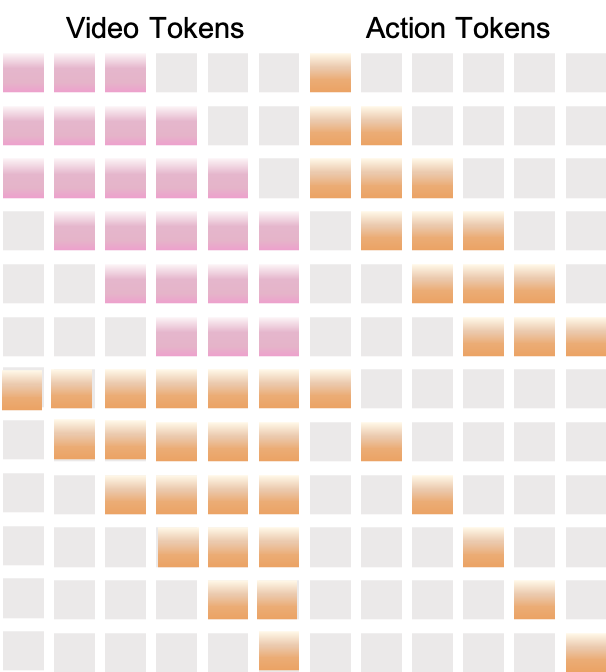
\includegraphics[width=0.5\linewidth]{assets/contextual_mask2.png}
  \caption{Contextual attention mask for GUIWorld.
  Video tokens (pink) and action tokens (orange) share one sequence.
  The mask restricts attention to a short temporal window so each frame attends only to nearby frames and temporally aligned actions.}
  \label{fig:contextual-mask}
\end{figure}

\noindent\textbf{Injection schemes.}
The GUI experiments explore four conditioning schemes built on this encoder: \texttt{external}, \texttt{contextual}, \texttt{internal}, and \texttt{residual} (Figure~\ref{fig:action-injection}).
Representative action-driven metrics comparing these modes are reported in Table~\ref{tab:gui-action-ssim}.
Full metric definitions and the evaluation protocol are provided in Appendix~\ref{appendix:gui-metrics}.


\newpage
\section{Additional Visualizations}
\label{appendix:vis}
\subsection{CLIGen Visualizations}
\noindent This subsection consolidates \emph{all} CLIGen visualization pages referenced in the paper.
The main text keeps section-local thumbnail panels at the end of each visualization subsection, while full-size pages are collected here.

\noindent\textbf{(1) \cligenGeneralData{} visualizations.}
Qualitative samples highlight the breadth of real-world terminal dynamics captured in CLIGen (General): ANSI escape sequences that repaint regions with changing foreground/background colors, incremental command entry with syntax highlighting and cursor edits, classic shell prompts and system outputs, long-running jobs with rapidly scrolling and color-coded package logs, full-screen TUIs, and progress dashboards.

\noindent\textbf{(2) \cligenCleanData{} REPL visualizations.}
In contrast to open-world traces, CLIGen (Clean) REPL samples are scripted and temporally well-paced (Figures~\ref{fig:cligen-clean-viz-a}--\ref{fig:cligen-clean-viz-d}; additional format examples are in Appendix~\ref{appendix:cligen-samples}). Each sample includes an explicit action trace (e.g., \texttt{Sleep}, \texttt{Type}, \texttt{Enter}, arrow keys, \texttt{Hide}) alongside rendered terminal frames, making action-to-pixel causality easy to inspect.

\noindent\textbf{(3) \cligenCleanData{} math visualizations.}
Figures~\ref{fig:cligen-clean-math-comp-a}--\ref{fig:cligen-clean-math-comp-c} compare model rollouts on CLIGen (Clean) math REPL prompts. Figures~\ref{fig:cligen-clean-math-rep-a}--\ref{fig:cligen-clean-math-rep-c} show reprompting cases and highlight why these probes should separate native computation from answer-conditioned rendering.

\subsection{GUIWorld Visualizations}
\noindent This subsection consolidates \emph{all} GUIWorld rollout visualizations (Figures~\ref{fig:guiworld-sample-1}--\ref{fig:guiworld-sample-14}).
CUA-based pages overlay the CUA trace (natural-language rationale when available, e.g., in a \texttt{thinking} field, plus structured \emph{action} fields such as \texttt{left\_click}, \texttt{double\_click}, \texttt{left\_click\_drag}, and \texttt{type}).
It contrasts the \emph{Ground Truth} trajectory (top) with a \emph{Generation} conditioned on the first frame and the action sequence (bottom), making state drift easy to spot.

Figures~\ref{fig:guiworld-sample-6}--\ref{fig:guiworld-sample-8} emphasize compounding low-level deviations; Figures~\ref{fig:guiworld-sample-9}--\ref{fig:guiworld-sample-11} focus on numeric/UI fidelity and interaction semantics; and Figures~\ref{fig:guiworld-sample-12}--\ref{fig:guiworld-sample-14} provide additional stress cases where correctness hinges on precise field edits and page state.

\newcommand{\BackToMainThumbs}[1]{%
  \hyperlink{#1}{%
    {\setlength{\fboxsep}{8.5pt}%
    \fcolorbox{metablue!55}{white}{\Large\bfseries\textsf{\strut Back to Main Thumbnails}}}%
  }%
}

\newcommand{\VisPage}[4]{%
  \clearpage
  \newgeometry{top=1.2cm,bottom=1.6cm,left=1.2cm,right=1.2cm,includefoot,footskip=22pt}
  \begin{landscape}
  \thispagestyle{plain}
  \noindent\makebox[\linewidth][r]{\BackToMainThumbs{#4}}\par
  \centering
  \vspace*{\fill}
  \includegraphics[width=0.98\linewidth,height=0.84\textheight,keepaspectratio]{#1}\par
  {\captionsetup{type=figure,skip=2pt}\captionof{figure}{#2}\label{#3}}
  \vspace*{\fill}
  \end{landscape}
  \restoregeometry
}

% CLIGen (General)
\VisPage{assets/cligen_general_1.pdf}{\cligenGeneralData{} visualization samples (A).}{fig:cligen-general-viz-1}{main-cligen-vis-thumbs-p1}
\VisPage{assets/cligen_general_2.pdf}{\cligenGeneralData{} visualization samples (B).}{fig:cligen-general-viz-2}{main-cligen-vis-thumbs-p1}
\VisPage{assets/cligen_general_3.pdf}{\cligenGeneralData{} visualization samples (C).}{fig:cligen-general-viz-3}{main-cligen-vis-thumbs-p1}

% CLIGen (Clean) REPL
\VisPage{assets/cligen_clean_1.pdf}{\cligenCleanData{} REPL visualization samples (A).}{fig:cligen-clean-viz-a}{main-cligen-vis-thumbs-p2}
\VisPage{assets/cligen_clean_2.pdf}{\cligenCleanData{} REPL visualization samples (B).}{fig:cligen-clean-viz-b}{main-cligen-vis-thumbs-p2}
\VisPage{assets/cligen_clean_3.pdf}{\cligenCleanData{} REPL visualization samples (C).}{fig:cligen-clean-viz-c}{main-cligen-vis-thumbs-p2}
\VisPage{assets/cligen_clean_4.pdf}{\cligenCleanData{} REPL visualization samples (D).}{fig:cligen-clean-viz-d}{main-cligen-vis-thumbs-p2}

% CLIGen (Clean) math comparisons
\VisPage{assets/cligen_math_comp1.pdf}{\cligenCleanData{} math comparison samples (A).}{fig:cligen-clean-math-comp-a}{main-cligen-vis-thumbs-p3}
\VisPage{assets/cligen_math_comp2.pdf}{\cligenCleanData{} math comparison samples (B).}{fig:cligen-clean-math-comp-b}{main-cligen-vis-thumbs-p3}
\VisPage{assets/cligen_math_comp3.pdf}{\cligenCleanData{} math comparison samples (C).}{fig:cligen-clean-math-comp-c}{main-cligen-vis-thumbs-p3}

% CLIGen (Clean) reprompting
\VisPage{assets/cligen_math_rep1.pdf}{\cligenCleanData{} math reprompting samples (A).}{fig:cligen-clean-math-rep-a}{main-cligen-vis-thumbs-p4}
\VisPage{assets/cligen_math_rep2.pdf}{\cligenCleanData{} math reprompting samples (B).}{fig:cligen-clean-math-rep-b}{main-cligen-vis-thumbs-p4}
\VisPage{assets/cligen_math_rep3.pdf}{\cligenCleanData{} math reprompting samples (C).}{fig:cligen-clean-math-rep-c}{main-cligen-vis-thumbs-p4}

% GUIWorld
\VisPage{assets/guiworld_sample_1.pdf}{\guiworldLogo{}\,GUIWorld visualization sample (1).}{fig:guiworld-sample-1}{main-gui-vis-thumbs-p1}
\VisPage{assets/guiworld_sample_2.pdf}{\guiworldLogo{}\,GUIWorld visualization sample (2).}{fig:guiworld-sample-2}{main-gui-vis-thumbs-p1}
\VisPage{assets/guiworld_sample_3.pdf}{\guiworldLogo{}\,GUIWorld visualization sample (3).}{fig:guiworld-sample-3}{main-gui-vis-thumbs-p1}
\VisPage{assets/guiworld_sample_4.pdf}{\guiworldLogo{}\,GUIWorld visualization sample (4).}{fig:guiworld-sample-4}{main-gui-vis-thumbs-p1}
\VisPage{assets/guiworld_sample_5.pdf}{\guiworldLogo{}\,GUIWorld visualization sample (5).}{fig:guiworld-sample-5}{main-gui-vis-thumbs-p1}
\VisPage{assets/guiworld_sample_6.pdf}{\guiworldLogo{}\,GUIWorld visualization sample (6).}{fig:guiworld-sample-6}{main-gui-vis-thumbs-p2}
\VisPage{assets/guiworld_sample_7.pdf}{\guiworldLogo{}\,GUIWorld visualization sample (7).}{fig:guiworld-sample-7}{main-gui-vis-thumbs-p2}
\VisPage{assets/guiworld_sample_8.pdf}{\guiworldLogo{}\,GUIWorld visualization sample (8).}{fig:guiworld-sample-8}{main-gui-vis-thumbs-p2}
\VisPage{assets/guiworld_sample_9.pdf}{\guiworldLogo{}\,GUIWorld visualization sample (9).}{fig:guiworld-sample-9}{main-gui-vis-thumbs-p2}
\VisPage{assets/guiworld_sample_10.pdf}{\guiworldLogo{}\,GUIWorld visualization sample (10).}{fig:guiworld-sample-10}{main-gui-vis-thumbs-p2}
\VisPage{assets/guiworld_sample_11.pdf}{\guiworldLogo{}\,GUIWorld visualization sample (11).}{fig:guiworld-sample-11}{main-gui-vis-thumbs-p3}
\VisPage{assets/guiworld_sample_12.pdf}{\guiworldLogo{}\,GUIWorld visualization sample (12).}{fig:guiworld-sample-12}{main-gui-vis-thumbs-p3}
\VisPage{assets/guiworld_sample_13.pdf}{\guiworldLogo{}\,GUIWorld visualization sample (13).}{fig:guiworld-sample-13}{main-gui-vis-thumbs-p4}
\VisPage{assets/guiworld_sample_14.pdf}{\guiworldLogo{}\,GUIWorld visualization sample (14).}{fig:guiworld-sample-14}{main-gui-vis-thumbs-p5}






\end{document}
